%% For submission and review of your manuscript please change the
%% command to \documentclass[manuscript, screen, review]{acmart}.
%%
%% When submitting camera ready or to TAPS, please change the command
%% to \documentclass[sigconf]{acmart} or whichever template is required
%% for your publication.
%%
%%
\documentclass[sigconf,review]{acmart}
%\documentclass[conference]{IEEEtran}

%% \BibTeX command to typeset BibTeX logo in the docs
\AtBeginDocument{%
  \providecommand\BibTeX{{%
    Bib\TeX}}}
%\def\BibTeX{{\rm B\kern-.05em{\sc i\kern-.025em b}\kern-.08em
%    T\kern-.1667em\lower.7ex\hbox{E}\kern-.125emX}}

%%% Rights management information.  This information is sent to you
%%% when you complete the rights form.  These commands have SAMPLE
%%% values in them; it is your responsibility as an author to replace
%%% the commands and values with those provided to you when you
%%% complete the rights form.
\setcopyright{acmlicensed}
\copyrightyear{2026}
\acmYear{2026}
\acmDOI{XXXXXXX.XXXXXXX}
%%% These commands are for a PROCEEDINGS abstract or paper.
\acmConference[Conference acronym 'XX]{Make sure to enter the correct
  conference title from your rights confirmation email}{June 03--05,
  2018}{Woodstock, NY}
%%%
%%%  Uncomment \acmBooktitle if the title of the proceedings is different
%%%  from ``Proceedings of ...''!
%%%
%%%\acmBooktitle{Woodstock '18: ACM Symposium on Neural Gaze Detection,
%%%  June 03--05, 2018, Woodstock, NY}
\acmISBN{978-1-4503-XXXX-X/2026/xx}
%
%
%%%
%%% Submission ID.
%%% Use this when submitting an article to a sponsored event. You'll
%%% receive a unique submission ID from the organizers
%%% of the event, and this ID should be used as the parameter to this command.
%%%\acmSubmissionID{123-A56-BU3}
%
%%%
%%% For managing citations, it is recommended to use bibliography
%%% files in BibTeX format.
%%%
%%% You can then either use BibTeX with the ACM-Reference-Format style,
%%% or BibLaTeX with the acmnumeric or acmauthoryear sytles, that include
%%% support for advanced citation of software artefact from the
%%% biblatex-software package, also separately available on CTAN.
%%%
%%% Look at the sample-*-biblatex.tex files for templates showcasing
%%% the biblatex styles.
%%%
%
%%\citestyle{acmnumeric}

\usepackage{cite}
\usepackage{algorithmic}
\usepackage{amsmath}
%\usepackage[noamsfonts]{amssymb}
\usepackage{amsfonts}
%\usepackage{hyperref}
\usepackage{url}
%\usepackage{tcolorbox} 
%\usepackage{fullpage}
\usepackage{adjustbox}
%\usepackage{pifont}
\usepackage{makecell}
%\usepackage{float}  % in preamble
\usepackage{graphicx}
\usepackage{comment}
\usepackage{enumitem}
%\usepackage{floatrow}
\usepackage{textcomp}
\usepackage{wrapfig}
%\usepackage{lscape}
%\usepackage{rotating}
\usepackage{graphicx}
\usepackage{caption}
%\usepackage{upgreek}
\usepackage{gensymb}
\usepackage{tabularx}
%\usepackage{csquotes}
%\usepackage{pdfpages}
%\usepackage{lipsum}
\usepackage{booktabs}
%\usepackage{array}
%\usepackage{adjustbox}
%\usepackage{amssymb}
\usepackage{pifont}
\usepackage{xspace}
\usepackage{xcolor}
\usepackage{float}

\usepackage{fontawesome}
\usepackage{scalefnt}

\setlist{nosep,leftmargin=*}
\hypersetup
{
colorlinks,
urlcolor=[blue]
}

\newcommand{\trip}{TRIP\xspace}
\definecolor{darkgreen}{RGB}{0,150,0}
\newcommand{\cmark}{{\color{darkgreen}\ding{51}}}

\definecolor{darkred}{RGB}{200,0,0}
\newcommand{\xmark}{{\color{darkred}\ding{55}}}

%\newcommand{\comment}[1]{}
\newcommand{\ignore}[1]{}

\newcommand{\ab}[1]{\textcolor{red}{Arnab: #1}}
\newcommand{\ari}[1]{\textcolor{blue}{Arindam: #1}}
\newcommand{\sm}[1]{\textcolor{blue}{Shubhadip: #1}}
\newcommand{\nl}[1]{\textcolor{darkgreen}{Neelu: #1}}
\newcommand{\pri}[1]{\textcolor{orange}{Priyanshu: #1}}

\newcommand{\tabcaption}[1]{\vspace*{0mm}\caption{#1}\vspace*{-3mm}}
\newcommand{\figcaption}[1]{\vspace*{-1mm}\caption{#1}\vspace*{-3mm}}

\newcommand{\figwidth}{0.85\columnwidth}

\begin{document}

\title
{TRIP: Optimal Personalized Multi-day Itinerary with Multi-modal Transportation and Dynamic Re-planning}

%\renewcommand{\shorttitle}{Planning the Perfect Itinerary}

%%
%% The "author" command and its associated commands are used to define
%% the authors and their affiliations.
%% Of note is the shared affiliation of the first two authors, and the
%% "authornote" and "authornotemark" commands
%% used to denote shared contribution to the research.

%\author{Anonymous Authors}

\ignore{

\author{
\IEEEauthorblockN{Priyanshu Jha\IEEEauthorrefmark{1}}
\IEEEauthorblockA{\textit{Computer Science and Engineering} \\
\textit{Indian Institute of Technology Kanpur}\\
Kanpur, India \\
priyanshu.jha.1973@gmail.com
%ORCID
}
\and
\IEEEauthorblockN{Neelu Lalchandani\IEEEauthorrefmark{1}}
\IEEEauthorblockA{\textit{Computer Science and Engineering} \\
\textit{Indian Institute of Technology Kanpur}\\
Kanpur, India \\
neelulalchandani29@gmail.com
%ORCID
}
\and
\IEEEauthorblockN{Shubhadip Mitra}
\IEEEauthorblockA{\textit{Blue Yonder India Pvt. Ltd.} \\
\textit{Bengaluru}\\
Bengaluru, India \\
shubhadip.mitra@blueyonder.com}
\and
\IEEEauthorblockN{Arnab Bhattacharya}
\IEEEauthorblockA{\textit{Computer Science and Engineering} \\
\textit{Indian Institute of Technology Kanpur}\\
Kanpur, India \\
arnabb@cse.iitk.ac.in
%ORCID
\and
\IEEEauthorblockN{Oswald C}
\IEEEauthorblockA{\textit{Computer Science and Engineering} \\
\textit{National Institute of Technology Tiruchirappalli}\\
Tiruchirappalli, India \\
oswald@nitt.edu }
\and
\IEEEauthorblockN{Arindam Pal}
\IEEEauthorblockA{\textit{TechSoftX Corporation}\\
Sydney, NSW, Australia \\
arindamp@techsoftx.com.au}
\and
\IEEEauthorblockA{\IEEEauthorrefmark{1}Both authors contributed equally to this
work}
%\and
%\IEEEauthorblockA{\IEEEauthorrefmark{2}Computer}
}
}
}

%\ignore{

\author{Priyanshu Jha}
\email{priyanshu.jha.1973@gmail.com}
\affiliation{%
  \institution{Dept. of Computer Science and Engineering}
  \city{IIT Kanpur}
  \country{India}
}

\author{Neelu Lalchandani}
\email{neelulalchandani29@gmail.com}
\affiliation{%
  \institution{Dept. of Computer Science and Engineering}
  \city{IIT Kanpur}
  \country{India}
}

\author{Shubhadip Mitra}
\email{shubhadip.mitra@blueyonder.com}
\affiliation{%
  \institution{Blue Yonder India Pvt. Ltd.}
  \city{Bengaluru}
  \country{India}
}

\author{Arnab Bhattacharya}
\email{arnabb@cse.iitk.ac.in}
\affiliation{%
  \institution{Dept. of Computer Science and Engineering}
  \city{IIT Kanpur}
  \country{India}
}

\author{Oswald C}
\email{oswald@nitt.edu}
\affiliation{%
  \institution{Dept. of Computer Science and Engineering}
  \city{NIT Tiruchirappalli}
  \country{India}
}

\author{Arindam Pal}
\email{arindamp@techsoftx.com.au}
\affiliation

%\renewcommand{\shortauthors}{Trovato et al.}

%\author{Neelu Lalchandani, Priyanshu Jha, Shubhadip Mitra, Arindam Pal, Oswald C, Arnab Bhattacharya}

\begin{abstract}
	%
	Given a tourist who intends to visit a set of points of interest (POIs)
	spread across a geographical region, the \emph{trip itinerary planning}
	 problem aims to identify an \textit{optimal itinerary} that \textit{maximizes} the
	tourist's \emph{utility} under a specified cost and time budget. An itinerary is
	defined as an ordered sequence of POIs that adheres to the time and budget
	constraints. This problem is not only important for tourists, but also for
	tour planners that offer personalized trips as business. Although there are
	few prior works that have attempted to address the above problem, they allow
	limited flexibility in terms of accommodating multiple transportation modes, planning a multi-day itinerary that adheres to the operational schedule of the POIs, 
	re-planning the itinerary based on tourist's actual visit duration of the
	POIs and live traffic situation,  andcustomizing the itinerary based on the
	personalized constraints and the utility function chosen by the user. This
	work revisits this problem with the goal of overcoming the above
	limitations, thereby considering more realistic factors.
	%
	In particular, the proposed solution, named \textbf{TRIP (TRip Itinerary Planner)} allows the tourist to (1)~plan a \emph{multi-day
	itinerary} that considers the operational schedule of the POIs and user's choice of the start and the end time of the trip and the originating POI and the ending POI for each day;
 (2)~factor in \emph{multiple transportation modes} based on available
	cost and time budget; (3)~customize the itinerary by allowing the tourist to specify one or more \emph{personalized constraints} that include must-see constraints, ordering constraints and category constraints;
(4)~choose from a
	\emph{set of utility function variants} that best captures his/her travel
	experience;
(5)~\emph{dynamically} adjust the remaining itinerary based on the delays or early exits made during the previously visited POIs.
  The problem is modeled using a directed graph, where the nodes represent
	POIs and the edges represent the available transportation modes between each
	pair of POIs. The problem is solved using a \emph{mixed integer
	linear program (MILP)}. A comprehensive
	empirical evaluation over a real data set comprising of several popular
	tourist destinations demonstrate the efficacy and efficiency of the proposed
	solution.
	%
\end{abstract}



\maketitle

%\ccsdesc[500]{Do Not Use This Code~Generate the Correct Terms for Your Paper}
%\ccsdesc[300]{Do Not Use This Code~Generate the Correct Terms for Your Paper}
%\ccsdesc{Do Not Use This Code~Generate the Correct Terms for Your Paper}
%\ccsdesc[100]{Do Not Use This Code~Generate the Correct Terms for Your Paper}

%%
%% Keywords. The author(s) should pick words that accurately describe
%% the work being presented. Separate the keywords with commas.
%\keywords{Itinerary Planning, Graph Algorithms, Mathematical Programming, Optimization, Points of Interest}
%% A "teaser" image appears between the author and affiliation
%% information and the body of the document, and typically spans the
%% page.

%\begin{IEEEkeywords}
%Itinerary Planning, Graph Algorithms, Mathematical Programming, Optimization, Points of Interest
%\end{IEEEkeywords}

\section{Introduction}

Tourism is one of the most dynamic and rapidly growing sectors of the modern
economy. However, planning trips that offer a rich travel experience remains a
non-trivial problem. A tourist planning to visit a new city faces the problem of
planning a suitable \emph{itinerary} that maximizes her utility under a given
cost budget and time budget. Here, an itinerary refers to a sequence of
\emph{points of interest (POIs)}, along with the respective time of arrival and
departure for each POI such that each POI is visited at most once. With the
increasing number of tourists and the increased availability of spatio-temporal
data, there is growing research interest in planning the trip itinerary
\cite{li2016travel, gavalas2014survey, sylejmani2011survey}. This problem is
important not only for tourists, but also for tour planners that offer
personalized trips.

Traditionally, most tourist destinations offer a set of pre-defined itineraries
that do not necessarily fit directly within the tourists' schedule, cost budget,
and preferences. As digital tourism resources and urban mobility platforms grow,
tourists expect personalized, optimal, and efficient travel itineraries that
meet their needs, constraints, and resources. Such itineraries are challenging
to construct manually due to the underlying complexity arising due to the number
of POIs, varying travel costs and durations, entrance fees, opening hours, and
different user interests. This creates a need for intelligent
itinerary planning systems that can generate effective and personalized trip
itineraries that offer high utility, while being cognizant of the requirements
of tourists. Although there exist several prior works \cite{chen2014automatic,
vanzelst2016itinerary, taylor2018tour, vu2022branch,
panagiotakis2024expectation, liu2024personalized, rambha2024optimized,
lim2018personalized, bolzoni2014efficient}, they have several limitations. Some
key limitations include: (1) None of the existing works allow the tourist to
choose from multiple available transportation modes such as walking, taxi, or a
hybrid mode allowing usage of multiple transportation modes
\cite{chen2014automatic, taylor2018tour, vanzelst2016itinerary}. (2) Many
tourists spend more than a day at a given tourist destination. This scenario
ideally calls for a multi-day trip itinerary planning that is aware of opening
and closing days of each POI along with opening and closing time for each open
day. However, majority of the earlier studies focus only on single-day itinerary
planning \cite{taylor2018tour, vu2022branch, panagiotakis2024expectation}.
While it may be possible to combine multiple single day itineraries to generate
a multi-day itinerary, it is not guaranteed to be as cost-effective (as
demonstrated in Sec.~6). Further, earlier studies paid little attention to the
operational schedule (i.e., operational timings of each open day) of the POIs
\cite{chen2014automatic, vanzelst2016itinerary, taylor2018tour}. (3) Often there
are tourists with specific requirements and preferences based on their
priorities and interests. These requirements and preferences must be respected,
along with the tourist's cost budget and time availability constraints. However,
many existing itinerary planning solutions ignore this need to
\emph{personalize} trip itineraries \cite{rambha2024optimized, yu2017mining,
rani2018development, yu2014optimal}. (4) While traveling based on a planned
itinerary, often it is required to update the remaining itinerary based on
unexpected delays or early exits from the previously visited POIs. This demands
dynamically adjusting the remaining itinerary as deemed necessary. However, to
the best of our knowledge, none of the existing works address this requirement
\cite{chen2014automatic, taylor2018tour, vanzelst2016itinerary}.

Motivated by the above limitations, this work addresses the following itinerary planning problem: \emph{Given a tourist who intends to visit a set of POIs spread across a geographical region, how to  identify an optimal itinerary that maximizes the tourist's utility under a specified cost budget and respects her choices and availability schedule that may span multiple days?} The itinerary must adhere to the tourist's specified starting location and time, and ending location and time for each day of the trip. Additionally, it must consider the operational schedule (day and timings) of each POI. The itinerary should factor in the tourist's preferred mode of transportation such as only walking, only taxi, or a hybrid mode that uses both walking and taxi, as necessary. The cost of the itinerary comprises of two components: (a)~\textbf{Transportation cost}, i.e., the cost incurred in traveling, (b)~\textbf{Visiting cost}, i.e., the cost incurred due to entry fees at each POI. Similarly, the time incurred is due to two components: (a)~\textbf{Travel time} between POIs, and (b)~\textbf{Visiting time} in a POI. The tourist may also specify one or more personalized constraints that include the following: (a)~\textbf{Must-see constraints:} These constraints specify a set of POIs that should necessarily be part of the itinerary, (b)~\textbf{Ordering constraints:} These indicate relative ordering between two or more POIs in the itinerary, (c)~\textbf{Category constraints:} Based on the similarity of the POIs, they may be classified into one or more categories. For example, museums, lakes and temples could be a set of categories. The category constraints allow a tourist to specify a lower bound and an upper bound on the number of POIs she wants to visit from each category. For instance, a tourist may decide to visit at least one but at most two museums. 

Based on the feedback of previous tourists, each POI is assumed to have a user-rating and recommended visit duration. The utility of a tourist at a given POI depends on the fraction of recommended visit duration she actually spends at the given POI and its average user-rating. The utility of the itinerary is aggregate of the utilities derived at each visited POI. The proposed trip itinerary planning problem allows the tourist to choose from a set of three utility variants that best captures her travel experience. The first variant offers full utility at a POI only if the tourist spends at least the recommended visit duration at the given POI, and zero otherwise. The second variant offers utility that is proportional to the fraction of time that the tourist spends at the given POI w.r.t. its recommended visit duration, provided the tourist  spends at least a minimum specified time. While the first variant can be viewed as a binary step function, the second variant can be viewed as its continuous linear counterpart. The third variant is a multi-step utility function., i.e., a $t$-step utility function where $t \ge 3$. The goal is to maximize the chosen utility variant.

Additionally, if there are unplanned delays or early exits in the earlier part of the itinerary, it should be possible to dynamically update the remaining itinerary based on the remaining cost budget and time budget. Here it is important to note that the reported itinerary not only returns a sequence of POIs to be visited, but also determines the amount of time the tourist spends at each POI (that in turn affects her utility) along with the suitable transportation mode (if more than one transportation modes are available) which in turn affects the travel time and the travel cost of the itinerary.

To address the above problem, this work proposes a novel solution framework,  called \textbf{\trip (TRip Itinerary Planner)}.  Firstly, the problem is modeled as a directed multi-graph $G$ where each node corresponds to a POI, and each edge corresponds to a travel between an ordered pair of POIs using a specific transportation mode such as walking or taxi. If there are $k$ ($k \ge 1$) transportation modes available between a given pair of POIs, then there are exactly $k$ directed edges between the corresponding pair of nodes in $G$, where each edge corresponds to a specific transportation mode, along with the associated travel cost and travel time. Subsequently, the solution is modeled using a mixed integer linear program (MILP) that returns an optimal itinerary.

The major contributions of this work are summarized as follows:
%
\begin{enumerate}
\item \textbf{Optimal Multi-day Itinerary:} This work proposes a novel multi-day trip itinerary planning solution, named \trip~ that returns an optimal itinerary under the specified cost budget and time budget constraints, while factoring the operational schedule (i.e., operational hours of each open day) of each POI.
\item \textbf{Multimodal Tour:} To the best of our knowledge, this is the first work to consider multiple transportation modes such as only walking, only taxi, or an hybrid mode that uses both walking as well as taxi, while planning trip itineraries.
\item \textbf{Personalized Constraints:} The proposed solution framework allows the tourist to specify one or more personalized constraints in the form of must-see constraints, ordering constraints and category constraints, as described earlier.
\item \textbf{Utility Variants:} The \trip~ solution framework allows the tourist to choose an utility variant from a set of three utility variants that best models her travel experience, as discussed above. The itinerary that maximizes the chosen utility variant is reported as the solution.
\item \textbf{Dynamic Rerouting:} This is the first work that allows dynamic adjustment of the remaining itinerary based on unplanned delays or early exits experienced while visiting the previous POIs of the itinerary.
\item Empirical evaluation on several popular tourist destinations confirm the efficacy and efficiency of the proposed solution. 
%
\end{enumerate}

The rest of the paper is organized as follows. Section 2 states the trip itinerary planning problem. Section 3 presents the \trip solution framework. Section 5 describes how the proposed solution can be extended to handle user specified personalized constraints such as must-see constraints, ordering constraints and category constraints. Further, it also discusses how the \trip solution  can optimize other utility variants; and how it performs dynamic re-routing, if necessary. Section 6 presents the experimental results, and finally, Section 7 concludes the paper with directions of future work.

\section{Related Work}
\label{Rel_Work}

We have summarized the recently published relevant papers in Table~\ref{tab:otherworks}. We can see that \trip is the only multi-day itinerary planning solution to offer multimodal transportation, choice of multiple utility variants, and dynamic re-planning. The ability to handle personalized constraints in the form of must-see POIs, must-avoid POIs, category constraints, and ordering constraints makes it even better. We next discuss these works.
 
Chen et al.~\citep{chen2014automatic} gave a scalable method to plan multiday trips according to user preferences. The system returns itineraries with low computation time, trading off scalability and personalization for real-time planning. van Zelst \citep{vanzelst2016itinerary} proposed Integer Linear Programming (ILP) based individualized travel itineraries in urban environments. Taylor et al. \citep{taylor2018tour} studied the problem of integrating user-defined POIs in travel planning using Integer Linear Program. They introduced the \emph{TourMustSee} problem, which is a variation of the well-known Orienteering Problem \citep{golden1987orienteering}. They have considered maximizing utility function similar to our \emph{\trip} solution. However, they have considered only the walking mode of transport and did not factor in the cost budget. Vu et al.~\citep{vu2022branch} advanced the formulation of the Tourist Trip Design Problem (TTDP) by including multiple practical constraints but could not achieve multiple-period itineraries. Multiday itinerary planning solution have been studied by~\citep{chen2014automatic,vanzelst2016itinerary,liu2024personalized,rambha2024optimized}. However, rather than optimizing any utility functions, they optimize either cost or time.  

Costas Panagiotakis et. al. ~\citep{panagiotakis2024expectation} presented a deterministic solution using Expectation-Maximization (EM) to construct personalized trips. While their system is a good starting point for static Personalized Itinerary Recommendation (PIR), it lacks some practical considerations applicable to real-world systems. Specifically, the system does not dynamically update the itinerary based on real-time information, and does not support multiple transport modes. A holistic satisfaction model for tour itinerary recommendation was proposed in~\citep{liu2024personalized}. Our extension builds upon this basis with the addition of dynamic real-time travel data collected through Google APIs, facilitating adaptive itinerary revision; fractional POI visit support for light interaction; and multimodal travel modes for more realistic tourist mobility modeling. 


A solution for optimizing the costs of such itineraries using an integer programming model is proposed by~\citep{rambha2024optimized}. Although this work focuses on minimizing the cost budget, it lacks support for handling personalized constraints and dynamic itinerary generation. Another solution PERSTOUR personalizes the trip recommendation for tourists based on user interests, duration and frequency of visit~\citep{lim2018personalized}. Though they could consider POI popularity and user interest preferences, uncertainties in POI visit duration and arrival times have not been addressed. \citep{bolzoni2014efficient} proposed a more realistic approach by adding categories to POIs with maximal cardinality constraints, which, however, falls significantly short in handling multiple real-world constraints. A recent work by J. Liu et. al \citep{liu2025optimizing} proposed a Strategic and Crowd-Aware Itinerary Recommendation
(SCAIR) algorithm which integrates real-world crowd behavior into route planning to optimize group utility. Though the algorithm generates an itinerary for dynamic planning incorporating time budget alone, it severely lacks in considering multiple other factors mentioned in the table. 

Detailed reviews of previous work are available in~\citep{gavalas2014survey} and~\citep{sylejmani2011survey}.
Other notable related works include~\citep{zheng2021novel,yu2017mining,jiaoman2018travel,sylejmani2017planning,zografos2008algorithms,rani2018development,yu2014optimal,arora2024itinerary}. In contrast to earlier work, our proposed \trip solution is powered by a wide variety of superior planning capabilities such as multimodal transportation, multiday itinerary planning, choice of utility variants, dynamic adjustment of itinerary and ability to accommodate user-specified personalized constraints.


\section{The Trip Itinerary Planning Problem}
\label{sec:problem}

We now introduce the \emph{Trip Itinerary Planning (TRIP) Problem}.
We assume a city with different points of interest (POIs),
represented as a graph where each POI is a node.  Every pair of POIs
is connected by multiple edges that represent the mode of transport
from one POI to the other.  Thus, if there are two modes of
transport---walking and taxi---there will be two edges between every
pair of POIs.  The weights on an edge $e$ is a tuple $\langle t_e,
c_e \rangle$ that represent the time of travel and the cost of travel
respectively for the particular travel mode.  The time of travel is
typically measured using a constant speed.  Thus, the distance
between the pair of POIs is divided by the constant speed to convert it
to time.  Similarly, the taxi cost is computed using a fixed formula
on the distance.  For walking, the cost is $0$.  Each POI $v$ has a
tuple $\langle t_v, c_v, U_v \rangle$ associated with it that
represents the time it takes to visit the POI, the cost (entry fees,
etc.) and the utility a traveler gets by visiting the POI
respectively.  We get this information from \ab{how??}.  While the
time to visit may change from one traveler to another, in this work,
we keep this fixed.  We do, however, let the time of visit of a POI
vary (\ab{Sec.~\ref{dynamic}}) for a user, with the associated
utility also changing.  Additionally, a POI may have a feasible
time-interval of visit in a day (say, a sunset spot, which can be
visited only in the afternoon from 4-6 pm), beyond which visiting it
gives an utility of $0$.  Each POI is also marked with a category or type (e.g.,
park, museum, etc.).  Finally, we have a total time budget and a cost
budget.  Both the time and the cost budgets are spent in traveling as
well as visiting the POIs.  The objective of the \emph{TRIP} problem
is to \emph{find an itinerary}, i.e., a sequence of POIs, that
\emph{maximizes the total utlity} of visiting the POIs under the
given time and cost budget.  The itinerary is prepended by a source
point (e.g., a hotel or an airport) and appended by a destination
point (again, hotel, airport, etc.).  The time and cost to travel
from the source to the first POI and the from the last POI to the
destination has to be also taken into account.

An itinerary $I$ of $n$ POIs is, thus, represented as a sequence
%
\begin{align}
	I = [ S, v_1, \dots, v_n, D ]
\end{align}
%
The total time spent for itinerary $I$ is
%
\begin{align}
	t(I) = t_{S,v_1} + t_{v_1} + t_{v_1,v_2} + t_{v_2} + \dots + t_{v_{n-1,v_n}} + t_{v_n} + t_{v_n,D}
\end{align}
%
which takes into account both the travel time and visiting time.  Similarly,
the total cost of itinerary $I$ is 
%
\begin{align}
	c(I) = c_{S,v_1} + c_{v_1} + c_{v_1,v_2} + c_{v_2} + \dots + c_{v_{n-1,v_n}} + c_{v_n} + c_{v_n,D}
\end{align}
%
which again takes into account both the travel time and visiting time.  The
utility obtained from $I$ is
%
\begin{align}
	U(I) = U_{v_1} + U_{v_2} + \dots + U_{v_n}
\end{align}
%
Given a time budget $T$ and a cost budget $C$, the TRIP problem is to find the
itinerary $I$ that maximizes $U(I)$ subject to the budget constraints:
%
\begin{align}
	& \arg\max_I U(I) \\
	\text{subject to } & t(I) \leq T \text{ and } c(I) \leq C
\end{align}

The traveler may put additional constraints on the itinerary such as
a particular POI must be visited (e.g., Eiffel Tower in Paris).  She
may also put restrictions in the form that not more than $k$ POIs of
the same category may be included and/or at least one POI of a particular
category must be included, etc.  She may also put in ordering
constraints, such as a temple must be visited before a museum, etc.  The feasible itinerary $I$ must satisfy all these
constraints.

\ignore{

In this work, we introduce the \emph{Trip Itinerary Planning (TRIP) Problem},
which is formulated as follows. The city is represented as a multimodal graph
of points of interest (POIs), with every pair of POIs connected by two edges
corresponding to walking and taxi travel. The taxi speed is $s_t$ and walking
speed is $s_w$. Using these, the time to travel from one POI to another is
calculated. Similarly, there is a cost per distance unit $c_t$ for taxi (the
corresponding cost for walking is $c_w = 0$), using which the cost of traveling
from one POI to another is computed. Every POI has a \emph{utility score},
which is its relative attractiveness or significance to the tourist. Given a
cost and a time budget, the basic problem is to \emph{find an itinerary}, i.e.,
a sequence of POIs, that \emph{maximizes the overall utility} obtained from the
chosen POIs. The core of the system is formulated as a Mixed-Integer Linear
Programming (MILP) problem, solved using the Gurobi Optimizer\footnote{\ab{cite
the tool}}, a powerful tool for mathematical optimization.
%The goal of the MILP model is to maximize the total utility obtained from the
%chosen POIs in the resulting itinerary, subject to a rich set of real-world
%constraints.

The itinerary is a linear, day-wise sequence of POIs that the tourist traverses
in the city over multiple days, while adhering to daily time constraints and
overall cost constraint. Let $V$ denote the set of POIs in the city. Each POI
has its associated opening and closing time, i.e., the time window in which it
can be explored by the tourists. Also, each POI has a weekly schedule and
specific operating days on which it can be visited.

\ab{This section is too much to-and-fro; there is not much of a flow -- we need to discuss}

Each POI \( v_i \in V \) has the following features:

\begin{itemize}
    \item \( U(v_i) \): Utility Score associated with each POI
    \item \( ot(v_i) \): Opening time of POI
    \item \( ct(v_i) \): Closing time of POI
    \item \( t(v_i) \): Average visit time spent by tourists on the POI
    \item \( c(v_i) \): Entrance fee for the POI.
\end{itemize}

\noindent \textbf{Multimodal Graph Representation:}
This problem is modeled using a multimodal graph \( G = (V, E) \) where:

\begin{itemize}
    \item \( V = \{v_1, ..., v_N\} \) denotes the set of all Points of interest of the city
    \item \( E \) contains two distinct edges between every pair of POIs \( (v_i, v_j) \), corresponding the two modes of travel:
    \begin{itemize}
        \item \textbf{Walking Edge} \( e^{w}_{i,j} \) is characterized by:
        \begin{itemize}
            \item \( t^{w}_{i,j} \): Time required to walk from \( v_i \) to \( v_j \).
            \item \( c^{w}_{i,j} \): Cost associated with walking (usually zero).
        \end{itemize}
        \item \textbf{Taxi Edge} \( e^{t}_{i,j} \) is characterized by:
        \begin{itemize}
            \item \( t^{t}_{i,j} \): Time required to travel by taxi.
            \item \( c^{t}_{i,j} \): Cost of travel by taxi.
        \end{itemize}
    \end{itemize}
    \item \textit{days} is the set of all days.
\end{itemize}

\noindent \textbf{Objective Function}\\
To create multi-day itinerary, the optimization ensures a balanced distribution across all days. The objective is to \textbf{maximize the total utility score across all days}.

The decision variable \( y_{i,d} \in \{0,1\} \) indicates whether POI \( v_i \) is selected on day \( d \). The objective function is:
\begin{align}
U(I) &= \sum_{d \in \text{days}} \sum_{i = 1}^{N} U(v_i) \cdot y_{i,d} \label{eq:multi_day_binary}
\end{align}

This equation computes the total utility $U(I)$ of the multi-day itinerary by summing the utilities of all selected POIs across all days.

The basic constraints of the system are described below:

\begin{itemize}

\item \textbf{Time Budget Constraint}\\
This constraint ensures that the total time taken i.e. the sum of visit and travel times is under the user specified time budget for each day.

\begin{align}
\label{mul_day_9}
    & \sum_{i \ne j} t^{w}_{i,j} \cdot w_{i,j,d}
    + \sum_{i \ne j} t^{t}_{i,j} \cdot x_{i,j,d}
    + \sum_{i \in V} t(v_i) \cdot y_{i,d} \leq H
\end{align}

where H is the time budget specified by user. The user can specify different time budgets for the first day, last day, and intermediate days to account for flight or train arrival and departure timings.
\\[1ex]
\item \textbf{Cost Budget Constraint} \\
 This constraint ensures that the total cost of the trip, including both taxi travel and POI entry fees, remains within the cost budget specified by the user.

\begin{align}
\label{mul_day_25}
\sum_{d \in \text{days}} \sum_{(i,j) \in I} \left(c^{w}_{i,j} \cdot w_{i,j} + c^{t}_{i,j} \cdot x_{i,j} \right) + \sum_{d \in \text{days}} \sum_{i \in I} c(v_i) \leq B 
\end{align}
where B is the cost budget for whole trip.
\\[1ex]
\item \textbf{Opening and Closing Time}\\
    This constraint makes sure that each POI is visited correctly in its operating hours:
    \begin{equation}
    \label{mul_day_29}
    s_{i,d} \geq \text{ot}_i \quad \forall i \in \text{{poi\_ids}}, \forall d \in \text{days} \\
    \end{equation}
    \begin{equation}
    \label{mul_day_30}
        s_{i,d} \leq \text{ct}_i - t(v_i) \quad \forall i \in \text{{poi\_ids}}, \forall d \in \text{days}
    \end{equation}
    \noindent
    where \( s_{i,d} \) is the arrival time at POI \( i \) on day \( d \)
\\[1ex]
\item \textbf{Opening and Closing Day}\\
    This constraint checks the availability of each POI on the day selected by the user. If the POI is not open for public during that day, then this constraint effectively uses $y[i, d] = 0$, to deliberately not include that POI in that day's itinerary.
    \begin{align}
    \label{mul_day_31}
 \quad y_{i,d} = 0 \quad  &\forall i \in \text{POI\_IDs}, \nonumber \\
        &\forall d \in \text{days, } \texttt{day\_availability}[\texttt{trip\_weekdays}[d]][i] = 0 \nonumber
\end{align}
    % \[\quad \forall i \in \text{{poi\_ids}}, \forall d \in \text{Days},\]
    \noindent
    where:
    \begin{itemize}
        \item \textit{days} represent the set of weekdays.
        \item \( \texttt{trip\_weekdays}[d] \) denotes the weekday corresponding to day \( d \).
        \item \( \texttt{day\_availability}[weekday][i] \) is 1 if POI \( i \) is open on that weekday, and 0 if it is closed.
    \end{itemize}
\end{itemize}

\textbf{Example}

}

\begin{figure}[t]
	\centering
	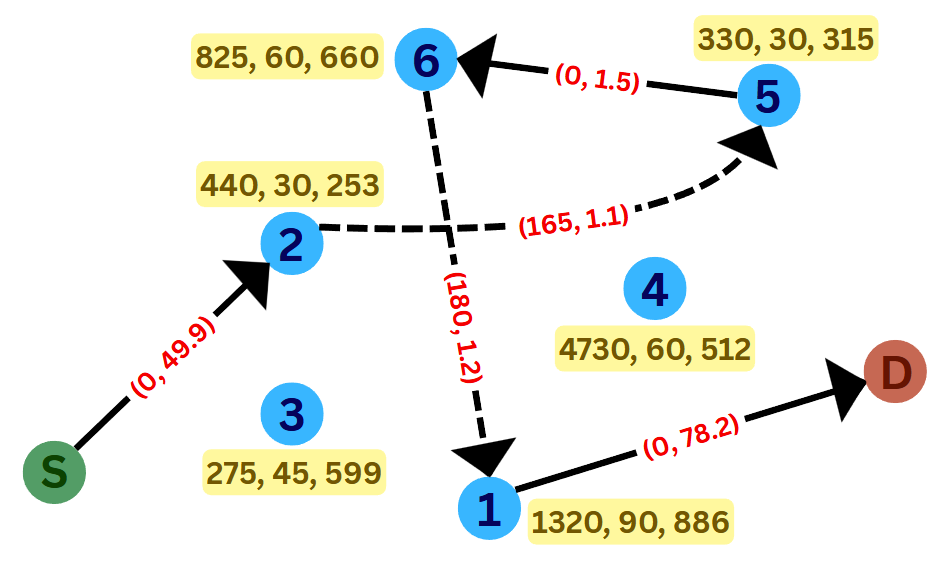
\includegraphics[width=0.75\columnwidth]{plots/updatedExample.png}
	\caption{Example: Solid Edges represent walking and Dashed edges represent Taxi, Edge labels depict \{travel cost, travel time\} and Vertex labels depict \{Visit cost, Visit  time, Utility score\}}
	\label{fig:example_graph}
\end{figure}

Consider an example of a city that has 6 POIs.
Table~\ref{tab:example_poi} shows the various time and cost values for
the POIs while Table~\ref{tab:example_walk} and
Table~\ref{tab:example_taxi} shows the travel times among the POIs and
the source and destination marked by $S$ and $D$ respectively for
walking and taxi respectively.

\begin{table}[t]
	\centering
	\resizebox{0.85\columnwidth}{!}
	{
		\begin{tabular}{c l rrr}
			\toprule
			\textbf{ID} & \textbf{Category} & \textbf{Visit Time} & \textbf{Utility} & \textbf{Visit Cost} \\
			\midrule
			%S & Source      & 0  & 0   & 0    \\
			1 & Park        & 90 & 886 & 1320 \\
			2 & Park        & 30 & 253 & 440  \\
			3 & Park        & 45 & 599 & 275  \\
			4 & Museum      & 60 & 512 & 4730 \\
			5 & Museum      & 30 & 315 & 330  \\
			6 & Museum      & 60 & 660 & 825  \\
			%D & Destination & 0  & 0   & 0    \\
			\bottomrule
		\end{tabular}
	}
	\caption{Details of Points of Interests (POIs)}
	\label{tab:example_poi}
\end{table}

\begin{table}[t]
	\centering
	\resizebox{\columnwidth}{!}
	{
		\begin{tabular}{c|cccccccc}
			\toprule
			\textbf{From$\backslash$To} & \textbf{S} & \textbf{1} & \textbf{2} & \textbf{3} & \textbf{4} & \textbf{5} & \textbf{6} & \textbf{D} \\
			\midrule
			\textbf{S} & --    & 28.7  & 49.9  & 55.5  & 68.9  & 126.6 & 117.2 & 102.9 \\
			\textbf{1} & 28.7  & --    & 3.3   & 3.2   & 4.3   & 10.1  & 9.3   & 78.2  \\
			\textbf{2} & 49.9  & 3.3   & --    & 5.7   & 2.7   & 8.0   & 6.9   & 94.3  \\
			\textbf{3} & 55.5  & 3.2   & 5.7   & --    & 5.0   & 9.9   & 9.6   & 47.4  \\
			\textbf{4} & 68.9  & 4.3   & 2.7   & 5.0   & --    & 5.8   & 5.0   & 74.7  \\
			\textbf{5} & 126.6 & 10.1  & 8.0   & 9.9   & 5.8   & --    & 1.5   & 98.5  \\
			\textbf{6} & 117.2 & 9.3   & 6.9   & 9.6   & 5.0   & 1.5   & --    & 102.4 \\
			\textbf{D} & 102.9 & 78.2  & 94.3  & 47.4  & 74.7  & 98.5  & 102.4 & --    \\
			\bottomrule
		\end{tabular}
	}
	\caption{Walking Travel Time Matrix}
	\label{tab:example_walk}
\end{table}

\begin{table}[t]
	\centering
	\resizebox{\columnwidth}{!}
	{
		\begin{tabular}{c|cccccccc}
			\toprule
			\textbf{From$\backslash$To} & \textbf{S} & \textbf{1} & \textbf{2} & \textbf{3} & \textbf{4} & \textbf{5} & \textbf{6} & \textbf{D} \\
			\midrule
			\textbf{S} & --    & 3.8  & 6.7  & 7.4  & 9.2  & 16.9 & 15.6 & 13.7 \\
			\textbf{1} & 3.8   & --   & 0.4  & 0.4  & 0.6  & 1.3  & 1.2  & 10.4 \\
			\textbf{2} & 6.7   & 0.4  & --   & 0.8  & 0.4  & 1.1  & 0.9  & 12.6 \\
			\textbf{3} & 7.4   & 0.4  & 0.8  & --   & 0.7  & 1.3  & 1.3  & 6.3  \\
			\textbf{4} & 9.2   & 0.6  & 0.4  & 0.7  & --   & 0.8  & 0.7  & 10.0 \\
			\textbf{5} & 16.9  & 1.3  & 1.1  & 1.3  & 0.8  & --   & 0.2  & 13.1 \\
			\textbf{6} & 15.6  & 1.2  & 0.9  & 1.3  & 0.7  & 0.2  & --   & 13.7 \\
			\textbf{D} & 13.7  & 10.4 & 12.6 & 6.3  & 10.0 & 13.1 & 13.7 & --   \\
			\bottomrule
		\end{tabular}
	}
	\caption{Taxi Travel Time Matrix}
	\label{tab:example_taxi}
\end{table}

Suppose a traveler has a time and cost budget of 360 and 3500 units respectively.
Additionally, she puts in the contraints that (1)~POIs 1 and 2 must be visited, (2)~POI 2 must be visited before POI 1, and (3)~POI 3, if visited, must be before both POI 2 and POI 5 (if visited).
Further, she must visit at least 2 POIs of the category Park, and will not visit more than 2 POIs of the category Museum.

Respecting all these constraints, the optimal itinerary is $[S, 2, 5, 6, 1, D]$, as shown in Figure~\ref{fig:example_graph}.  Note that the
POIs 3 and 4 were not included.  The total utility obtained from the
itinerary is 2114 units, and the time and cost spent in the itinerary
are, respectively, $341.9 (<360)$ and $3260 (<3500)$ units.
\ab{change the numbers!} \ari{Done!}

\ignore{

\textbf{Constraints applied:}
\begin{enumerate}[label=\textbf{\arabic*.}]
    \item \textbf{Time budget:} 360 minutes (5 hours)
    \item \textbf{Cost budget:} 3500 units
    \item \textbf{Must-see POIs:} POIs 1 and 2 must be included in the itinerary
    \item \textbf{Ordering constraints:} (Applied if both POIs are included in the itinerary)
    \begin{itemize}
        \item POI 3 must be visited before POI 2
        \item POI 2 must be visited before POI 1
        \item POI 3 must be visited before POI 5
    \end{itemize}
    \item \textbf{Category constraints:}
    \begin{itemize}
        \item At least 2 POIs from the \textit{Park} category
        \item At most 2 POIs from the \textit{Museum} category
    \end{itemize}
    \item \textbf{Modes of travel allowed:} Taxi and walking
\end{enumerate}
}


\section{The \trip Solution}
\label{sec:ilp}

In this section, we first outline the basic solution, before expanding it for
the different extensions.
Our solution is based on \emph{mixed integer linear programming} and is, hence,
\emph{optimal}.
In other words, no other algorithm can get a strictly better solution in terms
of utility with the given constraints.

\subsection{Basic Solution}
\label{sec:basic}

We propose a \emph{mixed integer linear programming (MILP)} solution for
the \trip problem.  Each POI $v_{j}$ is associated with a binary
variable $y_{j}$, which is $1$ if it is included in the optimal
itinerary, and $0$ otherwise.  Each edge (i.e., a connection between
POIs and the source and destination) between two POIs $v_{j}$ and
$v_{k}$ is also associated with an edge binary variable $z_{j,k}$; it is
$1$ if the edge is chosen, and $0$ otherwise.  To denote $m$ different
transport modes, $z$ is superscripted with the mode.  Thus, walking,
taxi, etc. are denoted as $z^1$, $z^2$, etc.  Assuming the city has $N$
POIs, without loss of generality, we treat the source $S$ and
destination $D$ as POI $v_{0}$ and $v_{{N+1}}$ respectively for uniform
treatment.  The cost and time of visit of a POI $v_i$ is denoted by
$c_i$ and $t_i$ respectively, while the cost and time of traveling from
POI $j$ to POI $k$ is denoted by $c_{j,k}$ and $t_{j,k}$ respectively.
In addition, 
we introduce an \emph{arrival time} variable for each POI, denoted by $a_i$ for node $v_i$.

\begin{figure}[t]
\begin{align}
	\label{eq:max}
	\max \quad & \sum_{\forall i} U_{{i}} \cdot y_{i} \\
	\text{subject to } \quad & \nonumber \\
	\label{eq:y}
	y_{i} & \in \{ 0, 1 \}, \forall i \\
	\label{eq:z}
	z^m_{j,k} & \in \{ 0, 1 \}, \forall j,k, \forall m \\
	\label{eq:sd}
	y_{0} = y_{{N+1}} & = 1 \\
	\label{eq:cost}
	\sum_{\forall j, k, \forall m} c_{{j},{k}} \cdot z^m_{j,k} + \sum_{\forall i} c_{i} \cdot y_{i} & \leq C \\
	\label{eq:time}
	\sum_{\forall j, k, \forall m} t_{{j},{k}} \cdot z^m_{j,k} + \sum_{\forall i} t_{i} \cdot y_{i} & \leq T \\
	\label{eq:sout}
	\sum_{\forall k} z^m_{{0},{k}} & = 1, \forall m \\
	\label{eq:sin}
	\sum_{\forall j} z^m_{{j},{0}} & = 0, \forall m \\
	\label{eq:din}
	\sum_{\forall j} z^m_{{j},{N+1}} & = 1, \forall m \\
	\label{eq:dout}
	\sum_{\forall k} z^m_{{N+1},{k}} & = 0, \forall m \\
	\label{eq:out}
	\sum_{\forall j} z^m_{{j},{k}} & \leq 1, \forall k, \forall m \\
	\label{eq:in}
	\sum_{\forall k} z^m_{{j},{k}} & \leq 1, \forall j, \forall m \\
	\label{eq:mode}
	\sum_{\forall m} z^m_{{j},{k}} & \leq 1, \forall j, k \\
	\label{eq:connectivity}
	\sum_{\forall j, \forall m} z^m_{{j},{i}} = \sum_{\forall k, \forall m} z^m_{{i},{k}} & = y_i, \forall i \\
	\label{eq:nodechosen1}
	\sum_{\forall m} z^m_{{j},{k}} & \leq y_j, \forall j,k \\
	\label{eq:nodechosen2}
	\sum_{\forall m} z^m_{{j},{k}} & \leq y_k, \forall j,k \\
	\label{eq:edgechosen1}
	\sum_{\forall k, \forall m} z^m_{{j},{k}} & \geq y_j, \forall j \\
	\label{eq:edgechosen2}
    \sum_{\forall j, \forall m} z^m_{{j},{k}} & \geq y_k, \forall k \\
	\label{eq:self}
	z^m_{{i},{i}} & = 0, \forall i, \forall m  \\
	\label{eq:subtour}
	a_j + (t_{j} + t_{j,k}) \cdot z_{j,k} & \leq a_k, \forall j,k
\end{align}
	\figcaption{Basic mixed integer linear programming solution}
\label{fig:basic}
\end{figure}

Fig.~\ref{fig:basic} outlines the equations for the
MILP solution for the basic \trip problem.  Eq.~\eqref{eq:max}
represents the \emph{utility maximization} problem, where the
utility of a POI $i$ is denoted by $U_i$.  Eq.~\eqref{eq:y} marks
the choice of POIs chosen for the optimal itinerary; however,
Eq.~\eqref{eq:sd} mandates the choice of the source and destination.
Eq.~\eqref{eq:z} marks the choice of edges for the optimal
itinerary.  Eq.~\eqref{eq:cost} and Eq.~\eqref{eq:time} put the
cost and time \emph{budget constraints} by adding up the
respective values for the POIs that are chosen (corresponding to
$y = 1$).  Eq.~\eqref{eq:sout} and Eq.~\eqref{eq:din} ensure that
the source and the destination is connected to one and only one
POI in the \emph{correct direction}, i.e., via one outgoing edge
and one incoming edge respectively only.  Eq.~\eqref{eq:sin} and
Eq.~\eqref{eq:dout} ensure that there is no incoming edge to the
source and no outgoing edge from the destination.
Eq.~\eqref{eq:out} and Eq.~\eqref{eq:in} constrain that each POI
has at most one incoming and at most one outgoing edge.
Eq.~\eqref{eq:mode} ensures that the chosen mode of travel is at
most one of the $m$ possibilities.  Eq.~\eqref{eq:connectivity}
imposes the \emph{connectivity constraint} by ensuring that a
node, if chosen, has exactly one incoming edge and an outgoing
edge.  Eq.~\eqref{eq:nodechosen1} and Eq.~\eqref{eq:nodechosen2}
imposes the condition that if a node is chosen, corresponding
edges in and out of it must be present as well.
Eq.~\eqref{eq:edgechosen1} and Eq.~\eqref{eq:edgechosen2} ensures
the opposite, i.e., if an edge is chosen, the corresponding nodes
are chosen as well.  Finally, Eq.~\eqref{eq:self} ensures that
there is \emph{no self-loop}.
Eq.~\eqref{eq:subtour} models an important constraint, that of \emph{subtour
elimination}.
Since the optimization is a \emph{maximization} problem, without this subtour
elimination constraint, the solution may include isolated cycles of POIs.
Eq.~\eqref{eq:subtour} prevents it by ensuring that if POI $k$ is visited
immediately after POI $j$, the start time of $v_k$ should be more than that of
$v_j$ plus the time of visit of $v_j$ and the travel time from $v_j$ to $v_k$.


%\section{Extensions of \trip}

\subsection{Personalized Constraints}
\label{sec:personalized}

We next the basic ILP problem, outlined in Eq.~\eqref{eq:max}--Eq.~\eqref{eq:self} to personalized constraints.

\subsubsection{Must-visit POIs}
\label{sec:must}

Suppose the traveler specifies a list of POIs $[m_1, \dots, m_k]$ that she
must visit.  Simply enforcing the corresponding $y$ binary variables to
$1$ ensures that these POIs are chosen in the optimal itinerary:
%
\begin{align}
	\label{eq:see}
	y_{m_i} & = 1, \forall i = 1, \dots, k
\end{align}

\subsubsection{Must-avoid POIs}
\label{sec:avoid}

Similarly, if the traveler explicitly lists a set of POIs $[a_1, \dots,
a_k]$ that she does not want to visit, the corresponding $y$ binary
variables are simply set to $0$:
%
\begin{align}
	\label{eq:avoid}
	y_{a_i} & = 0, \forall i = 1, \dots, k
\end{align}

\subsubsection{Category Constraints}
\label{sec:category}

To handle category contraints where a traveler specifies the range of
number of POIs that she wants to visit for a category, we augment the
variable $y$ associated with every POI with a category superscript.  For
example, if there are $l$ categories, the corresponding variables $y^1,
\dots, y^l$ represent the different possibilities.  If POI $i$ belongs to
category $k$, then, by definition, $y^j_i = 0, \forall j \neq k$, for
every other category $j$.  If every category $k$ has a lower bound $lb^k$
and upper bound $ub^k$ on number of POIs to be visited, then the basic
problem can be augmented by:
%
\begin{align}
	\label{eq:category}
	lb^k \leq \sum_{\forall i} y^k_i & \leq ub^k, \forall k
\end{align}
%
If the traveler only specifies the minimum number of POIs of a category
$k$ that she must visit, the upper bound $ub^k = N$; similarly, specifying
only the maximum number puts the lower bound as $lb^k = 0$.  For
categories where no constraint is mentioned, $lb^k = 0$ and $ub^k = N$.

\subsubsection{Ordering Constraints}
\label{eq:ordering}

A traveler can impose an ordering constraint, where she states that she will
visit POI $j$ before POI $k$, if the itinerary contains both of them.
To impose these ordering constraints, we introduce a \emph{start time} value for each POI, denoted by $s_i$ for node $v_i$.
%Correspondingly, an \emph{end time} value $e_i$ can be also declared.
If POI $j$ must be visited before POI $k$ (denoted as $j \prec k$), then $s_k$ must be after $s_j$ plus
the time it takes to visit $v_j$ (i.e., $t_{v_j}$) and the time it takes to
reach $v_k$ from $v_j$ (i.e., $t_{v_j,v_k}$).
Hence,
%
\begin{align}
	s_j + t_{j} + t_{j,k} & \leq s_k, \forall j \prec k
\end{align}
%
The above equation assumes that both POIs $j$ and $k$ are vsiited.
However, it may be the case that either $j$ or $k$ or both is not visited at all.
To handle the case that $j$ is not visited, the lower bound of $s_j$ for any
node is kept as $0$, and the times are added only if $y_j = 1$.
To handle the case that $k$ is not visited, a large value $M$ is added to $s_k$
when $y_k = 0$.
Together, the ordering constraint equation becomes
%
\begin{align}
	\label{eq:ordering}
	s_j + (t_{j} + t_{j,k}) \cdot y_j & \leq s_k + M \cdot (1 - y_k), \forall j \prec k
\end{align}
%

\subsection{POI Timings}

Many POIs have certain operating times.  For example, a temple may be open
only in the morning, from 9-11am.  Even otherwise, a traveler may specify that she wants to visit the temple in the morning hours only.  To handle this constraint, the start and
end time of the POI must be within this operational time.  Hence, if a POI
$i$ has an operational time denoted by entry and exit times $[en_i, ex_i]$,
then
%
\begin{align}
	\label{eq:operational}
	s_i \geq en_i \text{ and } & s_i + t_{i} \leq ex_i
\end{align}

\ignore{
		
\begin{itemize}

\item \textbf{Must-see POIs}\\
This constraint enforces that each POI marked as a must-see is visited exactly once over the duration of the trip:

\begin{equation}
\label{mul_day_7}
    \sum_{d \in \text{days}} y_{i,d} = 1 \quad \quad \forall i \in \text{must\_see\_pois}
\end{equation}

where:
\begin{itemize}
  \item \texttt{must\_see\_pois} is the set of user-specified must-visit POIs
\end{itemize}
\item \textbf{Must-avoid POIs}\\
This constraint enforces that each POI marked as excluded is never visited in the entire trip:

\begin{equation}
\label{mul_day_8}
    \sum_{d \in \text{days}} y_{i,d} = 0 \quad \quad \forall i \in \text{excluded\_pois}
\end{equation}

where:
\begin{itemize}
  \item \texttt{excluded\_pois} is the set of user-specified excluded POIs
\end{itemize}
\item \textbf{Category Constraints}\\
The user can specify the lower bound and upper bound for the categories of POIs to be visited across the trip. This constraint ensures that user's preferences over these themes are respected:

\begin{align}
\label{mul_day_11}
lb_m \leq \sum_{i \in V_m} \sum_{d \in \text{days}} y_{i,d} \leq ub_m, \quad \forall m \in C 
\end{align}

where:
\begin{itemize}
  \item \( C \) represents all the categories (e.g., historical, cultural, adventure, etc.)
  \item \( lb_m \) and \( ub_m \) are the lower and upper bounds for theme \( m \)
\end{itemize}

\item \textbf{Ordering Constraints}\\
If (a,b) is an ordering constraint, then POI a and POI b can be visited on different days, so this constraint makes sure that day of visit of POI a is before, or same as day of visit of POI b.
\begin{align}
\label{mul_day_12}
\texttt{day\_visit}_a \leq \texttt{day\_visit}_b, \quad \forall (v_a, v_b) \in P
\end{align}
\noindent
where:
\begin{itemize}
    \item \( \texttt{day\_visit}_a \): the day on which POI \( a \) is visited.
    \item \( P \): the set of all ordered POI pairs with ordering constraints entered by the tourist.
\end{itemize}

\item

\textbf{2. Intra-day Temporal Ordering Constraint}\\
If (a,b) is an ordering constraint and both POI a and POI b are to be visited on same day, then this constraint ensures that arrival time of POI b is greater than or equal to sum of arrival time of POI a, visit duration of POI a and travel time from POI a to POI b.

\begin{align}
\label{mul_day_13}
s_{i,d} + \left( t(v_i) + \left( t^{w}_{i,j} \cdot w_{i,j,d} + t^{t}_{i,j} \cdot x_{i,j,d} \right) \right) y_{i,d}
&\leq s_{j,d} + T_{ij} (1 - y_{j,d})\\ \forall (v_i, v_j) \in P,\; \forall d \in \text{days} \nonumber \\
\label{mul_day_14}
T_{ij} = ct(v_i) + t(v_i) + t^{w}_{i,j} 
\end{align}



\noindent
where:
\begin{itemize}
    \item \( s_{i,d} \): start time of visiting POI \( i \) on day \( d \).
    \item \( t(v_i) \):visit time spent at POI \( i \).
    \item \( ct(v_i) \): closing time of POI \(v_i\) \( i \).
\end{itemize}

\noindent
The Big-M term \( T_{ij} (1 - y_{j,d}) \) ensures the constraint becomes non-restrictive when POI \( j \) is not selected on day \( d \).
\end{itemize}

}

\subsection{Utility Variants}
\label{sec:utility}

The basic problem formulation assumes a traveler visits a POI for a fixed amount
of time, and gets the full utility offered by the POI.  However, in real life,
the time spent by every traveler is not the same.  Some may finish visiting a
POI in lesser time than the prescribed one, while some others may take longer
time.  In addition, some may not be willing to spend the full time in a POI, and
may sacrifice getting the full utility for partial utilization, and may come out
early to save time, and visit other POIs.  For example, a museum may have many
different types of rooms, such as sculpture, paintings, jewelry, etc., and a
traveler may not like to visit the jewelry section.  She may, thus, decide to
spend only a part of the total visit time for the other sections, get a partial
utility, and exit to go to another POI.  To capture this, we model the utility
in three variants:

\begin{enumerate}

	\item \textbf{Binary:} This is the standard utlity variant, where a
		traveler spends full time in a POI, and gets the complete utility.
		If she does not spend that time, she gets no utility at all. \ab{Is
		this right?}

	\item \textbf{Slab:} Here, the total visit time is divided into various
		slabs, starting from 50\%.  (We assume that a POI must be visited
		for at least 50\% of its time to get any utility.) Each slab is an
		interval of time spent as a percentage of the total visit time.
		When a traveler spends time in a slab of interval, she gets a
		percentage of utility equal to the lower end of the interval.
		Thus, if a slab is [60-70)\%, and a traveler spends 67\% time, she
		gets a utility equal to 60\% of the total utility.

	\item \textbf{Continuous:} The third variant models the utility as a
		continuous function equal to the percentage of time spent.  (Again,
		we impose the minimum time to be spent as 50\% for non-zero
		utility.) Thus, if a traveler spends 67\% time, she gets 67\%
		utility.

\end{enumerate}

Note that in all of these variants, if a traveler spends \emph{more} time
than the prescribed time of visit, her utility is capped to 100\% only.

The binary utility $U^b_i$ of a POI $i$ for the binary variant is captured
by the simple model: $U^b_i = U_i$.

For the slab variant, we divide the utility into 6 slabs: [50-60), [60-70),
[70-80), [80-90), [90-100), [100-$\infty$).  Correspondingly, we have 6 binary \emph{slab
variables} for every POI, $u^1, \dots, u^6$, with the constraint that at
most one of them is chosen (using the condition $\sum_{l=1}^6 u^l_i \leq 1$).  The \emph{effective
utility} of a POI $i$ is then:
%
\begin{align}
	\label{eq:slab}
	U^s_i = U_i \cdot ( & 0.5 \times u^1_i + 0.6 \times u^2_i + 0.7 \times u^3_i \nonumber \\
		& + 0.8 \times u^4_i + 0.9 \times u^5_i + 1.0 \times u^6_i )
\end{align}
%

The continuous variant introduces another variable $f_i$ to denote the fraction of time spent in a POI.
Its upper and lower bounds are set to 1.0 and 0.5 respectively.
The utility $U^c_i$ is simply $U^c_i = U_i \cdot f_i$.
\ab{how does it actually cap to 0.5 and 1.0?}

\ignore{

\noindent \textbf{Fractional Visits to POIs}\\
This feature enables partial visiting of Points of Interest (POIs), thus enhancing the flexibility and potential utility of the proposed itineraries. In comparison to the Binary approach used before which required the POI to be completely visited in order to collect its utility, the Fractional version built here grants proportional utility based on the proportion visited of the POI—improving time and cost budget efficiency.

\textbf{Fractional POI Variable (ppoi[i])}
\begin{itemize}
    \item A real variable $\text{ppoi}[i] \in [0, 1]$ is defined for every POI i to reflect the portion of the POI's total visit time covered by the itinerary.

    \item A threshold of 0.5 (50\%) is enforced: POIs must be visited for at least half of their average duration to be included. If ppoi[i] < 0.5, it is effectively set to 0 and the POI is excluded from the plan.
\end{itemize}

\textbf{Utility Calculation Variants}
\label{Utility_Calculation}

Two distinct methods are used to compute the utility in the fractional setting:

\begin{itemize}
\item {Continuous Linear Utility Model}

In this version, the utility granted is directly proportional to the fraction of the POI visited.

If a POI has utility $U$ and is visited for $p$ fraction of time (where $p \in [0.5, 1]$), the utility granted is $U \times p$.

\item{Slab-Based Utility Model}
\begin{itemize}[noitemsep, topsep=0pt]
    \item Fraction $\in$ [0.5, 0.6) $\rightarrow$ 50\% utility
    \item Fraction $\in$ [0.6, 0.7) $\rightarrow$ 60\% utility
    \item Fraction $\in$ [0.7, 0.8) $\rightarrow$ 70\% utility
    \item Fraction $\in$ [0.8, 0.9) $\rightarrow$ 80\% utility
    \item Fraction $\in$ [0.9, 1.0) $\rightarrow$ 90\% utility
    \item Fraction = 1.0 $\rightarrow$ 100\% utility
\end{itemize}

It is important to note that we provide 100\% utility if and only if POI is visited completely. The utility granted coincides with the lower bound because we do not want a situation like this to occur where even if we suggest that tourist visit 50\% POI and they get any utility greater than 50\% because that would scale up the actual utility as compared to the continuous linear function.
\end{itemize}

To enable fractional visits, the constraints were modified to make the visit duration at one POI proportional to a continuous variable \( ppoi_i \in [0,1] \), that represents the relative fraction of the overall visit duration spent at the POI \( v_i \). Accordingly, in all the constraints, the original visit times are multiplied by this fractional variable \( ppoi_i \), ensuring the constraints accurately reflect partial visits.

When the utility function is a continuous linear function of visit time, the utility score obtained from a POI is also scaled proportionally, i.e., \( \text{utility}_i = U(v_i) \cdot ppoi_i \), where \( U(v_i) \) is the full utility for a complete visit to POI \( v_i \).

For the slab-based utility variant, a continuous variable \( \text{effective\_utility}_i \) is used to capture the actual utility awarded based on the fraction of time spent at each POI. The utility is determined using discrete slab multipliers based on the visit duration. Each POI is assigned to at most one slab, and the utility is calculated as:

\begin{align}
\label{effective_utility}
\text{effective\_utility}_i &= U(v_i) \cdot \big(0.5 \cdot s_1[i] + 0.6 \cdot s_2[i] + 0.7 \cdot s_3[i] \notag \\
&\quad + 0.8 \cdot s_4[i] + 0.9 \cdot s_5[i] + 1.0 \cdot s_6[i] \big)
\end{align}

The optimization objective is to maximize the total utility accumulated across all POIs:

\begin{align}
\label{objective_fun_slabs}
U(I) = \sum_{i=1}^N \text{effective\_utility}_i
\end{align}

To ensure only one slab level is chosen per POI, the following constraint is imposed:

\begin{align}
\sum_{k=1}^{6} s_k[i] \leq 1, \quad \forall i \in \{1, \dots, N\}
\end{align}

}

\subsection{Multi-Day Itinerary}

For large tourist-forendly cities, covering all the POIs may not be
possible within a single day, and travelers typically look for
\emph{multi-day} tour itineraries.  Most work solve it trivially by first
running for a single-day, getting rid of the POIs covered in that day, and
then running again for the next day, and so on.  Instead, we solve the
problem as one single optimization problem.  For each day, we can specify a
source and destination, and the time budget.  This caters to tours where
the time in the first and last days are typically less due to arrival and
departure constraints.  Also, the first day's source and the last day's
destination may be an airport or a rail station, while for other days, it
is a hotel.

For an itinerary having $d$ days, we augment all the variables with a
superscript that indicates the day of the visit.  Thus, the $y$ and $z$
binary variables are replicated for each day: $y^d_i$ and $z^{m,d}_{j,k}$
for all POIs $i$, modes of transport $m$ and days of visit $d$.  While the
cost budget (Eq.~\eqref{eq:cost}) is imposed on the overall tour, the time
budget constraints (Eq.~\eqref{eq:time}) are imposed per day.  The rest of
the constraints--incoming, outgoing, mode, connectivity, nodechoice,
edgechoice, and no self loop--(Eq.~\eqref{eq:sout} to Eq.~\eqref{eq:self})
remain the same, and are applied for each day.  Additionally, the following
conditions ensure that a POI is chosen at most once within $d$ days:
%
\begin{align}
	\label{eq:multiday}
	\sum_{\forall d} y^d_i & \leq 1, \forall i
\end{align}
%
Choosing a POI at most once automatically constraints choosing any incoming
or outgoing edge to or from it to at most once as well.

\subsection{Dynamic Itinerary Re-planning}

So far, we have discussed only static plans.
Once an optimal tour is decided, it is not altered.
However, in real life, both tourist behavior as well as other conditions including weather, traffic, etc. are not deterministic in nature, and change over time.
To handle this, we introduce \emph{dynamic tour re-planning} where we keep computing the best tour given the current situation.
To the best of our knowledge, no other tour planner does that.

We initially start with an optimal static plan using our solver that takes into account the traveler's preferences.
However, after visit of every POI, we provide an option to her to \emph{re-optimize} the rest of the plan based on the current situation.
This may happen since she may have spent substantially less or more time in a POI, or the current traffic condition has somehow altered significantly due to accidents, etc.

Our solver now replans the schedule based on the remaining time and cost
budgets. The POIs already visited are not considered further (they are
added as must-avoid POIs), and the current POI is considered the source.
This optimizes the rest of the tour based on current progress and not
static assumptions.

\ignore{

The real tourist behavior and weather conditions, are dynamic and unpredictable in nature. They can be influenced by unforeseen delays, detours, longer-than-anticipated visits, or spontaneous user preferences, which can significantly impact the feasibility and correctness of an advanced preplanned itinerary. To close the gap between theory and practice, a dynamic approach is required.

In contrast with the static approach used in \cite{taylor2018tour}, where rigid, precomputed travel times and POI visit times, we have taken real-time travel times using Google-Maps API (Routes API). 

On the top of suggested times of visit and travel, user can enter the actual time they have taken to visit a POI and the travel time they took to reach the current POI.

With every visit to a POI, the system replans the schedule based on the remaining time and cost budgets. The POIs already visited are not considered for further itineraries. This optimizes the rest of the day based on current progress and not stale assumptions.

For the dynamic feature, a record of visited POIs was maintained. On visiting a POI, it was eliminated from the list to be taken into account in future itinerary calculations with the new remaining time and cost budgets.

}

\begin{figure}[th]
\textbf{Implementation of Dynamic Approach}
\centering
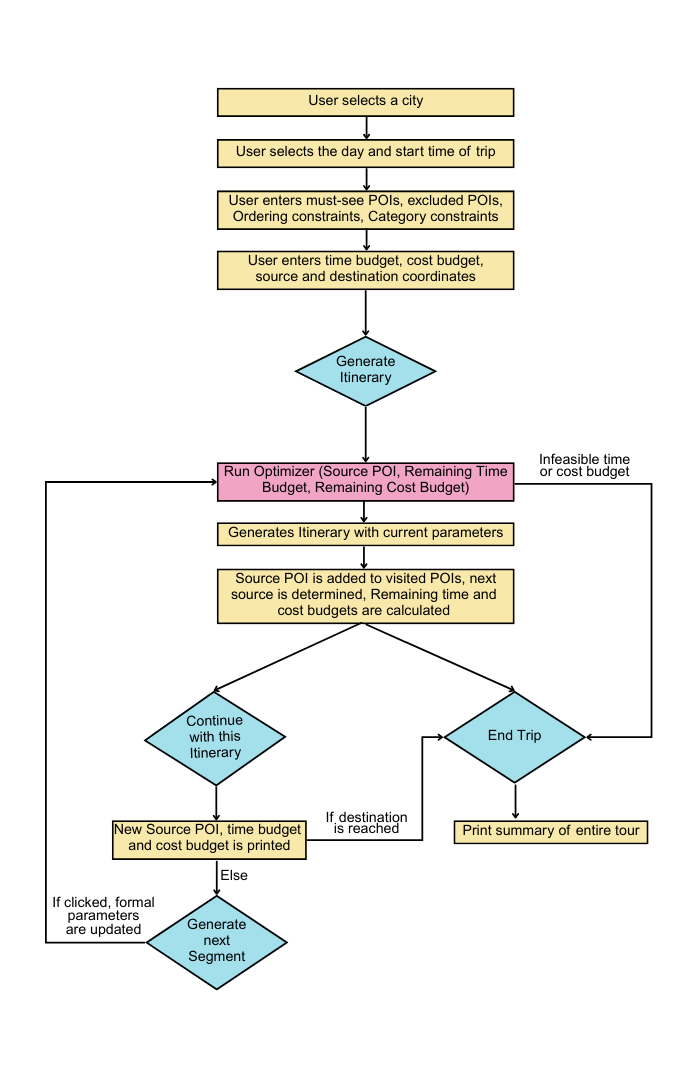
\includegraphics[width=0.5\textwidth]{binary dynamic flowchart.png}
	\caption{Implementation of Dynamic Approach -- \ab{is this figure needed? May be simplify}}
\label{fig:flowchart_dynamic}
\end{figure}


\section{Experiments}

\subsection{Dataset Description}
In order to test our itinerary planning system, we used curated datasets of Points of Interest (POIs) for seven large cities: Delhi, Budapest, Vienna, Osaka, Glasgow, Edinburgh, and Perth. \ari{Americans will be very unhappy.} The initial dataset utilized is derived from the \textbf{Yahoo Flickr Creative Commons 100 Million Dataset (YFCC100M)} \cite{}, \ari{Missing citation.} containing over 100 million images, of which 69 million are annotated and 48 million are geotagged. \ab{69+48>100.} \ari{Some of the images are common, i.e., both annotated and geotagged.}

We used the Flickr User-POI Visits dataset available at ~\cite{limkwanhuiDataCode}, \ab{are we using 2 separate datasets?} which was generated in the following manner. In order to generate this dataset, the authors of the paper ~\cite{taylor2018tour} took a set of popular POIs for every city mentioned earlier using resources such as \textit{Wikipedia}. Then, geotagged photos in \textit{Flickr} were matched with these POIs using spatial proximity. By estimating relative \textbf{popularity} of a POI through the counts of photos for every POI, the relative popularity which is referred to as utility was estimated.

This approach generates an empirical proxy for real tourist behavior, measuring interest in a specific attraction as measured by publicly accessible, crowd-sourced images.

The existing dataset contained the following key fields for each POI:

\begin{table}[th]
\begin{tabularx}{0.5\textwidth}{p{3cm} X}
\hline
\textbf{Field Name} & \textbf{Description} \\
\hline
\texttt{poiID} & A unique identifier assigned to each POI. \\
\hline
\texttt{poiName} & The name of the POI, e.g., ``Red Fort'', ``Osaka Castle''. \\
\hline
\texttt{lat} & Latitude coordinate of the POI. \\
\hline
\texttt{long} & Longitude coordinate of the POI. \\
\hline
\texttt{theme or category} & Thematic classification of the POI, such as \textit{amusement}, \textit{historical}, \textit{museum}, \textit{shopping}, \textit{park}, etc. \\
\hline
\texttt{Utility Score or Profit} & A numerical value representing the estimated utility or attractiveness of the POI, derived based on its popularity (photo frequency). \\
\hline
\texttt{Cost} & Geospatial travel distance (in meters) between pairs of POIs. This is used in the travel time estimation between locations, with the walking speed $v_w$ and taxi speed $v_t$. \\
\hline
\end{tabularx}
\caption{Original dataset fields}
\end{table}

\subsection{Experimental Setup}

With an aim to make our system more realistic and practical to use, we supplemented the dataset manually with real-life operating limitations and data that we gathered from \textbf{official tourist websites} and verified online portals. The added fields are:

\begin{table}[th]
\centering
\begin{tabularx}{0.5\textwidth}{p{3cm} X}
\toprule
\textbf{Field Name} & \textbf{Description} \\
\midrule
\texttt{fees} & Entrance fee or ticket price associated with the POI, in INR. \\
\midrule
\texttt{opening time} & The time at which the POI opens for visitors, stored in \texttt{HH:MM:SS} format. \\
\midrule
\texttt{closing time} & The time at which the POI closes for visitors, stored similarly. \\
\midrule
\texttt{Days of Week} & Seven binary columns (\texttt{Monday}, \texttt{Tuesday}, ..., \texttt{Sunday}). A value of 1 indicates the POI is open on that day; 0 indicates it is closed. \\
\midrule
\texttt{Avg Visiting Time} & The average duration (in minutes) tourists typically spend at the POI. \\
\bottomrule
\end{tabularx}
\caption{Additional features added to the dataset}
\end{table}

These manually extracted features add a \textbf{temporal and availability aspect} to the optimisation problem, allowing more realistic and accurate itinerary generation. For example, POIs closed on the chosen day are excluded from the planning automatically.

All the other information was collected by scraping or quoting \textbf{official tourist boards}, \textbf{city tourism websites}, and trustworthy travel websites.

\subsection{Configuration}

The experiments were conducted on a MacBook Air equipped with an Apple M1 processor and 8GB of RAM, providing a lightweight yet efficient environment for developing and testing the itinerary planning system. The implementation was carried out in Python, leveraging its rich ecosystem for data handling, user interaction, and visualization. The core optimization process was performed using the Gurobi Optimizer, a state-of-the-art solver for mathematical programming. Gurobi was employed to solve the underlying Integer Linear Programming (ILP) formulations that generate optimized multi-day travel itineraries under various user-defined constraints and real-world conditions.

\subsection{Baseline Itinerary Planner}

To establish a baseline for evaluation, we implemented the itinerary planning model described in Taylor and Lim \cite{taylor2018tour}, which we refer to as the \textbf{baseline model}. This model adopts a binary decision framework, where each Point of Interest (POI) is either fully included in the itinerary or completely excluded which is equivalent to our binary walking version of trip itinerary planner.

Although several works in this domain are summarized in Table~\ref{tab:otherworks} which can serve as a baseline, but none of them provided access to their code or implementation details. This made it non-trivial to reproduce their approaches based solely on the paper, as most did not even include the evaluation metrics used for comparison. Among them, the only paper that was somewhat implementable was the one published at \textit{WWW}. While it too lacked a code repository or implementation details like the detalils about the POI visiting durations used by the authors of the paper, we were able to replicate the key features and constraints described. In order to ensure a fair comparison, we repeatedly reached out to the authors of relevant baseline papers, seeking access to their implementation or reported results. Ultimately, we used the theoretical constraints outlined in their paper, along with the necessary baseline constraints for correctness, as a reference for evaluating our model.


\ignore{

The utility function in this setting is defined as:

\[
\max \left\{ \sum_{i=2}^{N} \sum_{j=2}^{N} S_i \cdot x_{i,j} \right\},
\]

where \( x_{i,j} = 1 \) if POI \( i \) is visited immediately before POI \( j \), and 0 otherwise. \ab{what is $s_i$?} This is equivalent to the binary utility formulation:

\[
\sum_{i=1}^{N} U(v_i) \cdot y_i
\]

where \( U(v_i) \) denotes the utility of POI \( v_i \), and \( y_i \in \{0,1\} \) is a binary variable indicating whether \( v_i \) is selected in the itinerary.
}

The baseline model incorporates only fundamental constraints, including the time budget constraint, connectivity requirements, a restriction preventing a direct path between the start and the end POIs, and  sub-tour elimination constraints which the authors mentioned in their paper. In our implementation, the sub-tour elimination is effectively enforced using arrival-time-based constraints. We were able to seamlessly adapt our ILP-based framework to replicate this baseline behavior, effectively converting our advanced planner into a simplified version matching the baseline model's structure.

However, direct performance comparison between our model and the baseline was not feasible due to a key limitation in the common dataset used by both our system and Taylor and Lim \cite{taylor2018tour} --namely, the absence of standardized POI visiting durations. Second, the baseline paper distributed POI visit durations by an unspecified method, making it impossible to reproduce exactly the same execution cases. Despite this, we were able to re-implement the baseline model in its entirety in terms of constraints as well as utility structure, which provided a good basis for qualitative analysis. 

Another limitation of the itinerary planner described in Taylor and Lim \cite{taylor2018tour} was that it did not consider any cost budget during itinerary planning. To address this, we incorporated cost constraints into our model. However, to ensure a fair comparison with their approach, we used a very high cost budget in our experiments so that it would not influence the itinerary planning outcome.


\ab{No mention of absence of cost budget}

\subsection{9 Variants of the \trip}

We evaluate the performance of the \trip solution by considering its variants as listed in Table~\ref{tab:trip_variants}, that are based on the transportation mode and the chosen utility variant. 
\begin{table}[th]
\centering
\begin{tabular}{|l|l|l|}
\hline
\textbf{TRIP VARIANT} & \textbf{Transportation Mode} & \textbf{Utility Variant} \\
\hline
TRIP\_W\_B & Walk & Binary \\
TRIP\_T\_B & Taxi & Binary \\
TRIP\_H\_B & Hybrid -- Walk + Taxi & Binary \\
TRIP\_W\_C & Walk & Fractional -- CLF \\
TRIP\_T\_C & Taxi & Fractional -- CLF \\
TRIP\_H\_C & Hybrid -- Walk + Taxi & Fractional -- CLF \\
TRIP\_W\_S & Walk & Fractional -- Slabs \\
TRIP\_T\_S & Taxi & Fractional -- Slabs \\
TRIP\_H\_S & Hybrid -- Walk + Taxi & Fractional -- Slabs \\
\hline
\end{tabular}
\caption{\trip Variants by Transportation Mode and Utility Variant}
\label{tab:trip_variants}
\end{table}


\subsection{Input Parameters and Performance Metrics}

\textbf{User Inputs}\\
Our trip planning system is capable of accepting a wide range of user inputs to support personalized and realistic trip planning. They are:

\begin{itemize}
    \item \textbf{City Choice:} The city would be selected by the user from options.
    
    \item \textbf{Trip Day:} The actual day on which the trip is to take place.

    \item \textbf{Start and End Points:} Latitude and longitude coordinates identifying the point where the day's journey begins and ends.
    
    \item \textbf{User Preferences:}
    \begin{itemize}
        \item \textbf{Category Constraints:} Limit on the category of POIs to be addressed, i.e., museum, market, park, etc.
        \item \textbf{Must-See and Must-Exclude POIs:} Individual POIs that the user must add or remove from the itinerary.
        \item \textbf{Ordering Constraints:} Ordering constraints with respect to POIs, indicating visit priority.
    \end{itemize}
    
	\item Utility Variant: \ab{Add the utility variants}
    \item \textbf{Time Budget:} The time (minutes or hours) the user is willing to spend on the trip.
    \item \textbf{Cost Budget:} The maximum cost which the user will incur on travel expenditure (e.g., taxi fares) and entry fees of POIs.
    
    \item \textbf{Dynamic Variant Specific Inputs:}
    \begin{itemize}
        \item \textbf{Actual Visitation Time per POI:} Used to update the remaining itinerary dynamically during execution.
        \item \textbf{Actual Travel Time between POIs:} Used to dynamically recalculate transitions and reschedule the visits accordingly.
    \end{itemize}
    
    \item \textbf{Multi-day Trip Specific Inputs:}
    \begin{itemize}
        \item \textbf{Number of Days:} Total number of days in the trip.
        \item \textbf{Start, End, and Hotel Coordinates:} Coordinates specifying the start, end, and overnight locations for each day.
        \item \textbf{Start, End, and Hotel Coordinates:} Coordinates that show the start, end, and overnight locations for every day.
        \item \textbf{Start Time \& Time Budget per Day:} Daily starting time and allowed time budget for each day, \\specified per day (first/last/intermediate day).
    \end{itemize}
\end{itemize}
\vspace{0.5cm}
\noindent\textbf{Performance Metrics}\\
We evaluate the quality and efficiency of the generated itineraries using the following performance metrics:

\begin{itemize}
    \item \textbf{Utility:} The total utility obtained from the selected POIs in the itinerary. It reflects how well the chosen points align with user preferences.
    
    \item \textbf{Running Time:} The time (in seconds) required by the system to compute the itinerary. It is an indicator of the system's computational efficiency.
    
    \item \textbf{Time Utilisation:} The percentage of the user-provided time budget that is actually used in the itinerary:
    \[
    \text{Time Utilisation \%} = \frac{\text{Total time used}}{\text{Time budget}} \times 100
    \]
    
    \item \textbf{Fraction of Time Spent in Travel and Visits:}
    \begin{itemize}
        \item \textbf{Travel Time Fraction:} Ratio of time spent traveling between POIs to the total available time.
        \item \textbf{Visit Time Fraction:} Ratio of time spent visiting POIs to the total available time.
    \end{itemize}
\end{itemize}

\ab{Add Cost Utilization}

These metrics serve as the basis for the comparative analysis and graphical illustrations presented in the subsequent section.

\subsection{Demonstrations}

To demonstrate the performance and insights of our itinerary planning system, we begin with a comprehensive visualization in Figure~\ref{fig:cities}, which presents the variation of utility across different time and cost budgets for all seven cities in our dataset. This offers a broad perspective on how the system adapts to varying resource constraints in diverse urban environments. For the remainder of the analysis, we focus on the city of Osaka as a representative case. Unless stated otherwise, the default time budget is varied within a practical range of 480 to 600 minutes, and the cost budget is chosen to be appropriately aligned with the economic characteristics of the city. This approach allows us to maintain clarity while drawing generalizable conclusions from representative trends observed in one city.

\newpage
\noindent \textbf{Comparison 9 variants with the Baseline Model}
\begin{figure}[th]
\centering
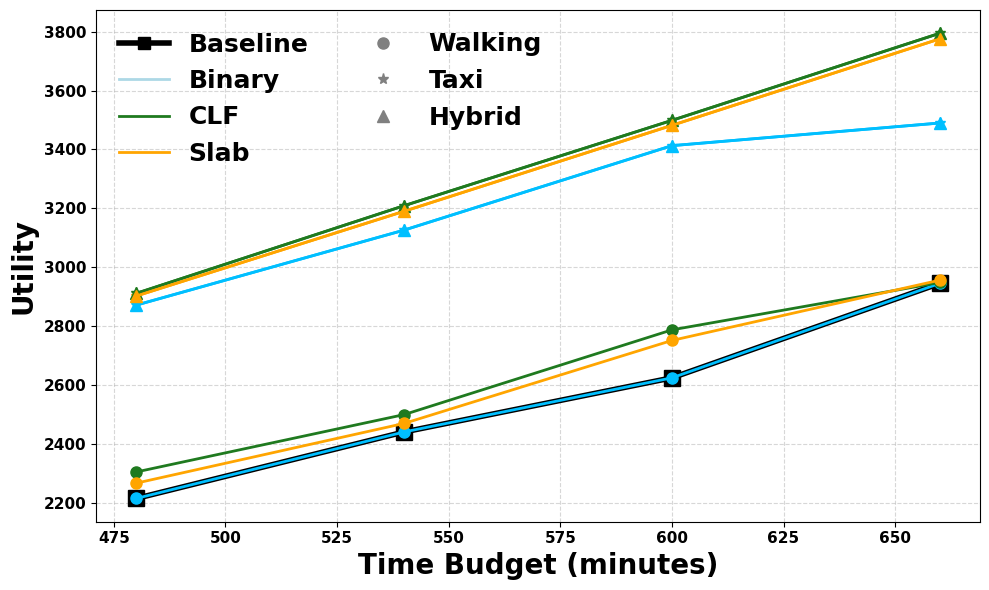
\includegraphics[width=0.5\textwidth]{plots/singledaycomparison.png}
\caption{Comparison of Single-day trips with Baseline Model}
\label{fig:comparisonWithBaselinePlot_singleday}
\end{figure}
\noindent
\textbf{Figure~\ref{fig:comparisonWithBaselinePlot_singleday}} illustrates the comparison of utility scores across different trip durations for various models under a high cost budget scenario (1,00,000 units). A clear upward trend is observed across all models, indicating that utility increases with longer trip durations—consistent with the intuitive understanding that more time allows for visiting more POIs.

Notably, the \textit{Binary-Walking} variant of our model closely replicates the behavior of the \textit{Baseline model}, validating its correctness and fairness for comparative purposes. However, our advanced models—especially those incorporating partial POI visits and additional travel modes such as \textit{Taxi} and \textit{Hybrid}—consistently outperform the baseline in terms of utility. Among these, the \textit{CLF (Continuous Linear Function)} utility model with \textit{Hybrid mode} demonstrates the highest utility scores, indicating the effectiveness of both the advanced utility formulation and flexible transport options in enhancing itinerary quality.

Interestingly, at the cost cap of 1,00,000 units, the utility scores of \textit{Taxi} and \textit{Hybrid} modes overlap, suggesting that under a relaxed cost constraint, both modes are able to achieve similar performance. This cost ceiling is deliberately set to eliminate cost-related influences, ensuring a fair comparison focused on time and utility behavior because the baseline model is not capable of handling cost related factors.

Overall, the plot effectively highlights how our approach—especially the allowance for partial POI visits and the use of flexible transport—leads to significantly improved itinerary recommendations, both in terms of utility and adaptability to real-world constraints.



\begin{figure}[th]
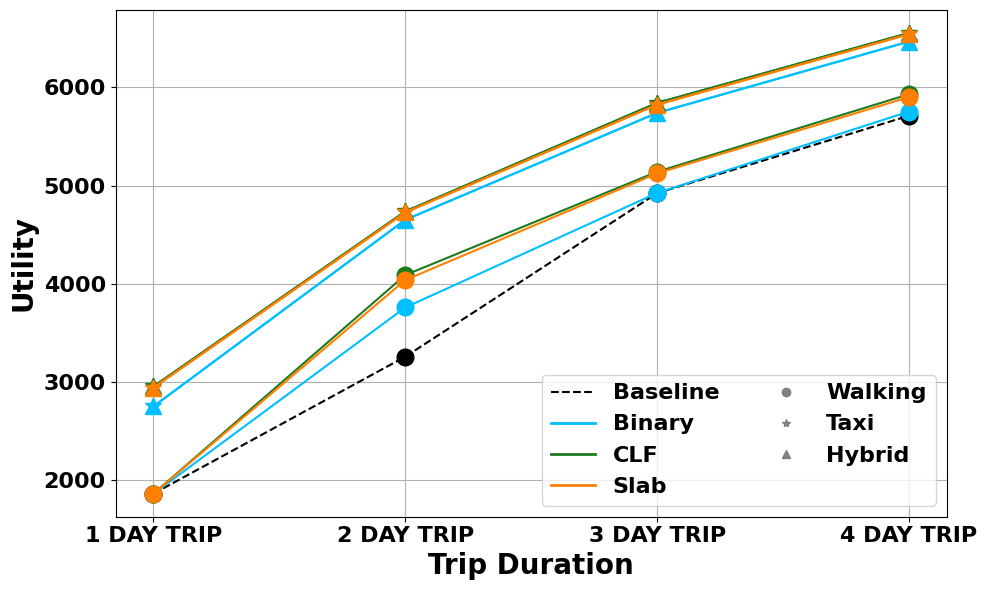
\includegraphics[width=0.5\textwidth]{plots/baselineComparison_pkj.png}
\caption{Comparison of Multi-day trips with Baseline Model}
\label{fig:comparisonWithBaselinePlot}
\end{figure}

The plot~\ref{fig:comparisonWithBaselinePlot} compares the performance of our proposed trip planning variants against a baseline model for trips ranging from one to four days. For a fair comparison, the time budget was fixed at 8 hours per day, and the cost budget was set high at 1,00,000 units - ensuring that cost wouldn’t be a limiting factor, especially for the baseline. The baseline utilities were calculated by creating daily itineraries one after another, making sure not to repeat any POIs from previous days, and summing up the utilities. On the other hand, the nine other variants represent results from our optimized multi-day planning models, which take a more holistic approach. As seen in the graph, all of our variants consistently outperform the baseline across all durations. Given this clear advantage, we have chosen to leave the baseline out of future comparisons to keep things focused. Moreover, this setup results in identical utility values for taxi and hybrid modes, as taxi usage becomes universally optimal due to its time-saving advantage when cost is not an issue. \\

\noindent\textbf{Effect of Multi-modality}

\begin{figure}[th]
\centering
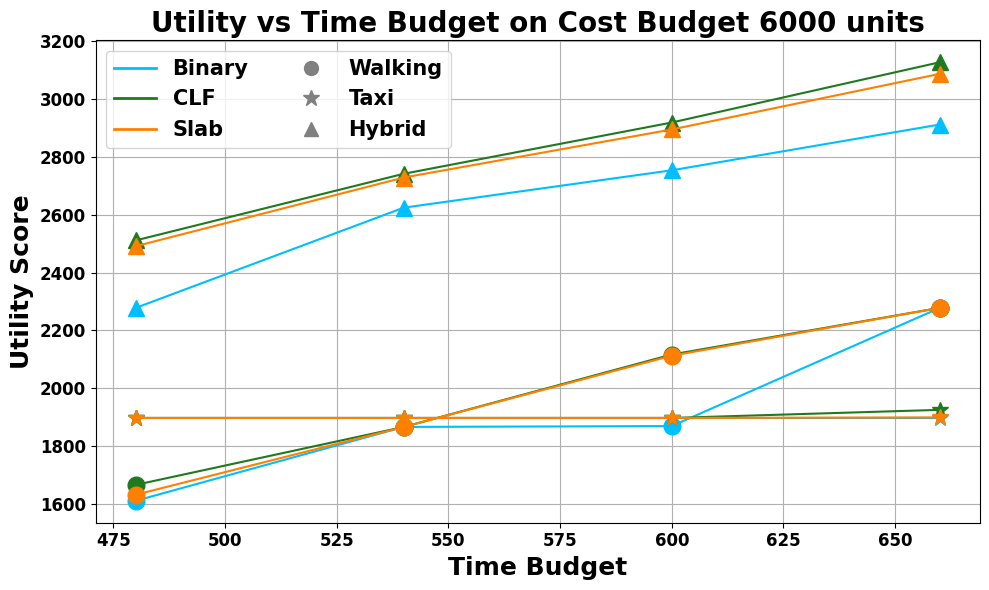
\includegraphics[width=0.45\textwidth]{plots/multimodality1.png}
\label{fig:mm1}
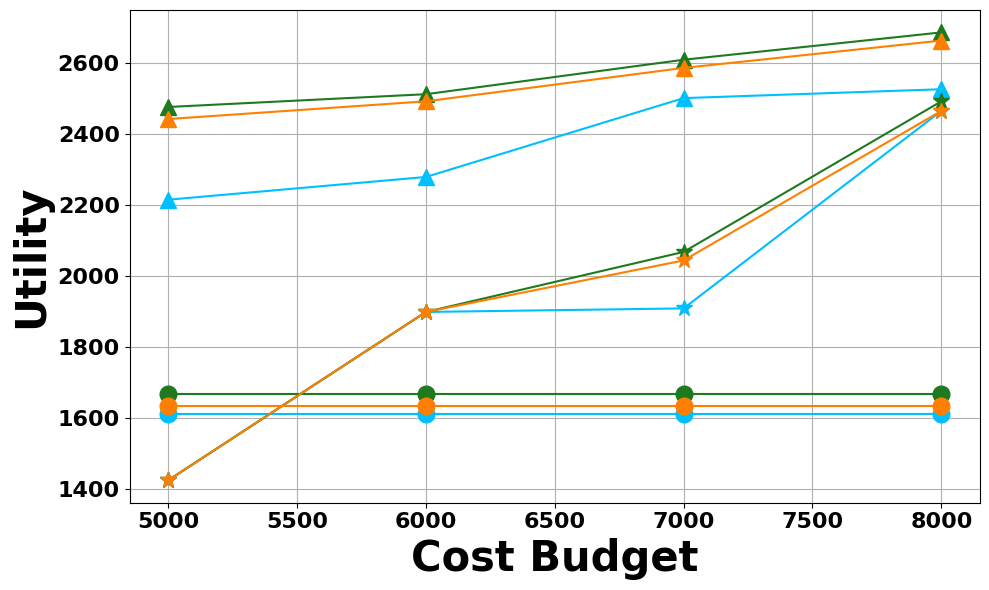
\includegraphics[width=0.45\textwidth]{plots/multimodality2.png}
\caption{Plots for variation of Utility in single-day trips in 9 variants at Cost Budget 6000 units and Time Budget 480 minutes respectively}
\label{fig:mm2}
\end{figure}

\noindent\textbf{Legend Description}\\
Figure ~\ref{fig:mm2}  distinguishes utility computation variants (B, C, S) using different line colors. The travel modes are represented by markers: circle for Walking, star for Taxi, and triangle for Hybrid mode. For instance, a blue star denotes $TRIP\_T\_B$ mode, orange triangle denotes $TRIP\_H\_S$ mode and so on.

This experiment was done to illustrate the impact of varying time and cost budgets on the utility achieved by different transportation modes in our itinerary planning framework. The top graph explores how increasing the time budget (with a fixed cost budget of 6000 units) affects utility. Here, we observe that the utility continues to increase for walking and hybrid modes, while it saturates for the taxi-only variant. This is because the taxi mode relies heavily on cost availability—once the fixed cost budget is consumed, additional time offers very little, to no further improvement. In contrast, the hybrid mode, which leverages both walking and taxi flexibly, consistently outperforms the single-mode options across all three TRIP variants, highlighting the effectiveness of our multi-modality feature.

The lower graph, which holds the time budget constant at 480 minutes while increasing the cost budget, further supports this observation: hybrid models adapt more efficiently to increased resource availability, maximizing utility better than single-mode approaches. In this case, the utility for walking-only variants remains saturated across all TRIP variants, as the potential gains from walking are constrained by the fixed time rather than by cost. Furthermore, a consistent trend is observed wherein the CLF (Continuous Linear Function) scoring model outperforms the slab-based model. This is because CLF assigns utility proportionally to the time spent at a POI—for example, visiting a POI for 63\% of its average duration yields 63\% utility—while the slab model would round this down to 60\% based on predefined thresholds, resulting in a measurable loss. Together, both graphs validate our design choices, demonstrating the combined advantages of multi-modal transportation and continuous utility modeling in enhancing itinerary quality.\\

\noindent\textbf{Time Utilization}
\begin{figure}[th]
\textbf{Travel Times vs Visit Times in different Modes and Cost Budgets- CLF Variant}\\
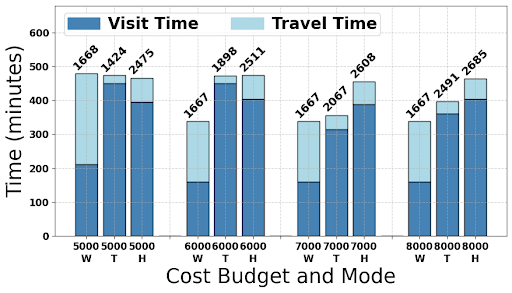
\includegraphics[width=0.5\textwidth]{plots/tu1.png}
\centering
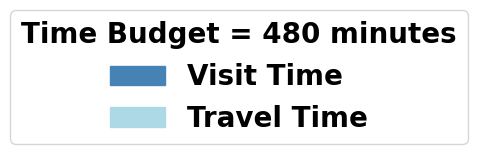
\includegraphics[width=0.25\textwidth]{plots/tu_legend1.png}
\caption{Time Utilization in 3 travel Modes on different cost budgets and fixed time budget (480 minutes)- Osaka}
\label{fig:TimeUtilization}
\end{figure}

\begin{figure}[th]
\textbf{Travel Times vs Visit Times in different Modes and Time Budgets - CLF Variant}\\
% 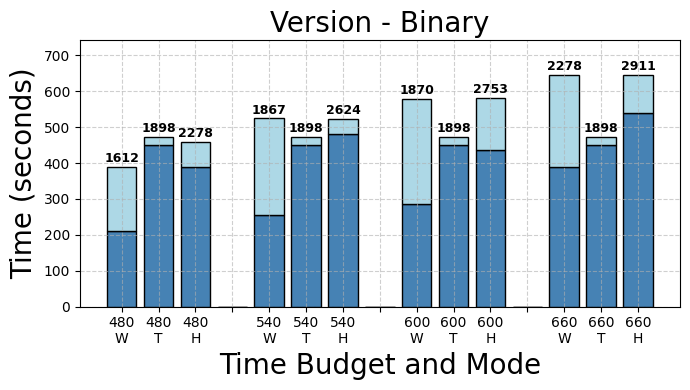
\includegraphics[width=0.23\textwidth]{plots/TIME_UTILIZATION_BINARY1.png}
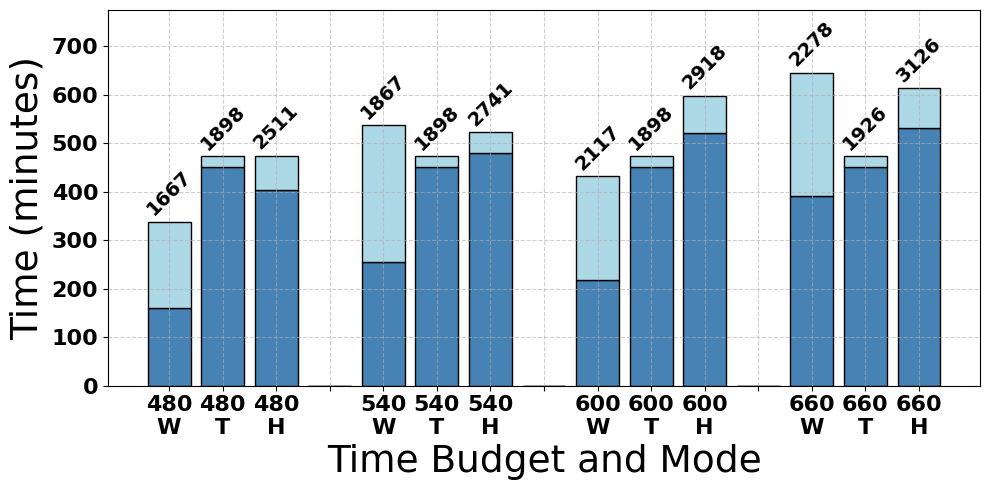
\includegraphics[width=0.5\textwidth]{plots/tu2.png}
% 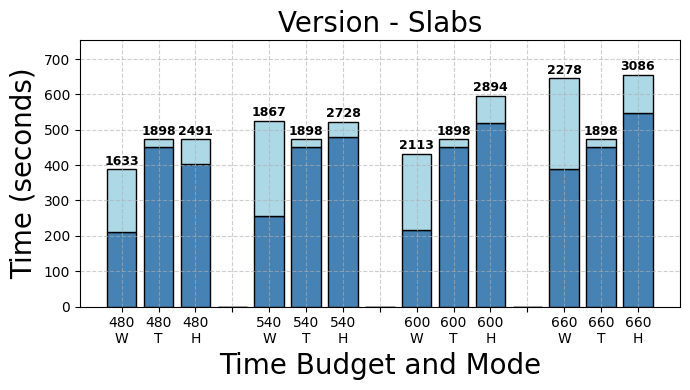
\includegraphics[width=0.23\textwidth]{plots/TIME_UTILIZATION_SLABS1.png}
\centering
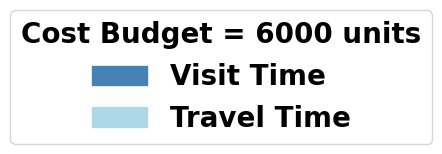
\includegraphics[width=0.25\textwidth]{plots/tu_legend2.png}
\caption{Time Utilization in 3 travel Modes on different time budgets and fixed cost budget (6000 rupees)- Osaka}
\label{fig:TimeUtilization1}
\end{figure}

Figures~\ref{fig:TimeUtilization} and ~\ref{fig:TimeUtilization1} present a comparison of travel time versus visit time across the three TRIP variants---walking-only (TRIP\_W), taxi-only (TRIP\_T), and hybrid (TRIP\_H)---at a fixed time budget of 480 minutes and varying cost budgets (5000, 6000, 7000, and 8000 units) and at a fixed cost budget of 6000 units and varying time budgets (480, 540, 600 and 660 minutes) respectively. Across all three utility scoring versions (B, C, and S), a clear trend emerges: TRIP\_W exhibits a high travel-to-visit time ratio, reflecting the slower nature of walking as a mode of transport. In contrast, TRIP\_T minimizes travel time due to exclusive reliance on taxis, thereby maximizing time spent at points of interest (POIs). The hybrid model, TRIP\_H, maintains a balanced ratio between travel and visit time, offering a compromise between the two extremes. While the taxi-only model may seem efficient in terms of maximizing visit time, earlier experiments have demonstrated that it is the hybrid TRIP\_H that achieves the highest overall utility. Across all variants, increasing time budget allowed better utilization of available time, with Hybrid mode consistently providing the most balanced performance across travel and visit times. This highlights that optimizing for utility involves not just maximizing visit duration but also strategically balancing travel efficiency with multi-modal flexibility.\\

\noindent\textbf{Cost Utilization}

\begin{figure}[th]
\textbf{Travel Cost vs Visit Cost in different Modes and Time Budgets}\\
% 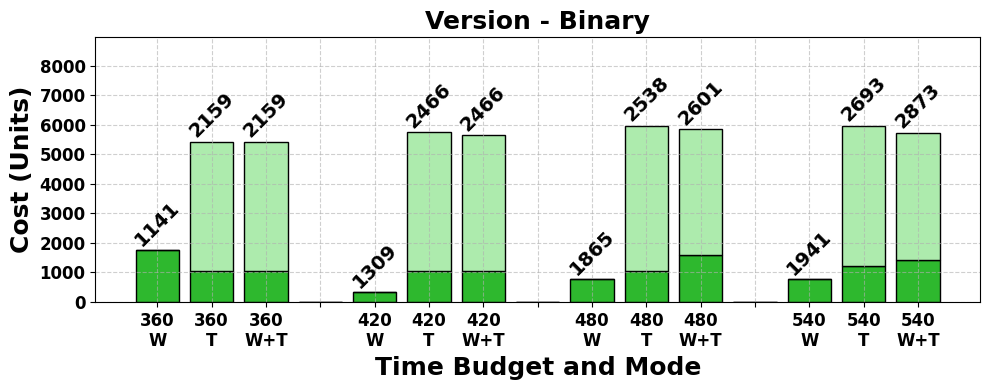
\includegraphics[width=0.5\textwidth]{plots/CU3_pkj.png}
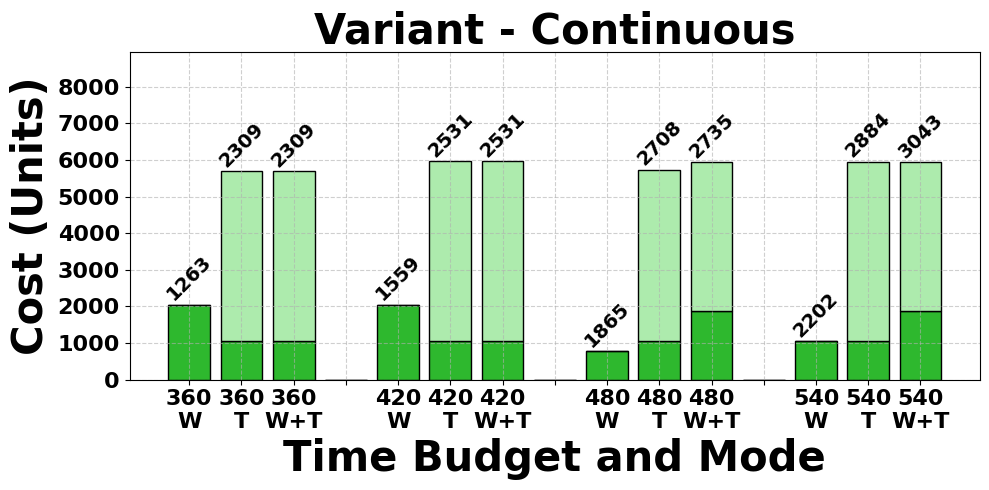
\includegraphics[width=0.5\textwidth]{plots/CU1.png}
% 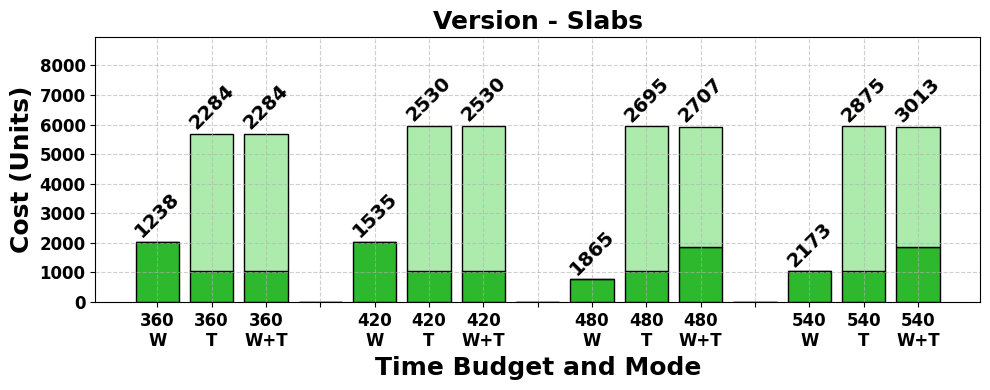
\includegraphics[width=0.5\textwidth]{plots/CU2_pkj.png}
\centering
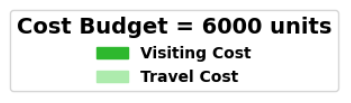
\includegraphics[width=0.3\textwidth]{plots/cu1_legend.png}
\caption{Cost Utilization in 3 travel Modes on different time budgets and fixed cost budget (6000 units)- Osaka}
\label{fig:CostUtilization1}
\end{figure}

\begin{figure}[th]
\textbf{Travel Cost vs Visit Cost in different Modes and Cost Budgets}\\
% 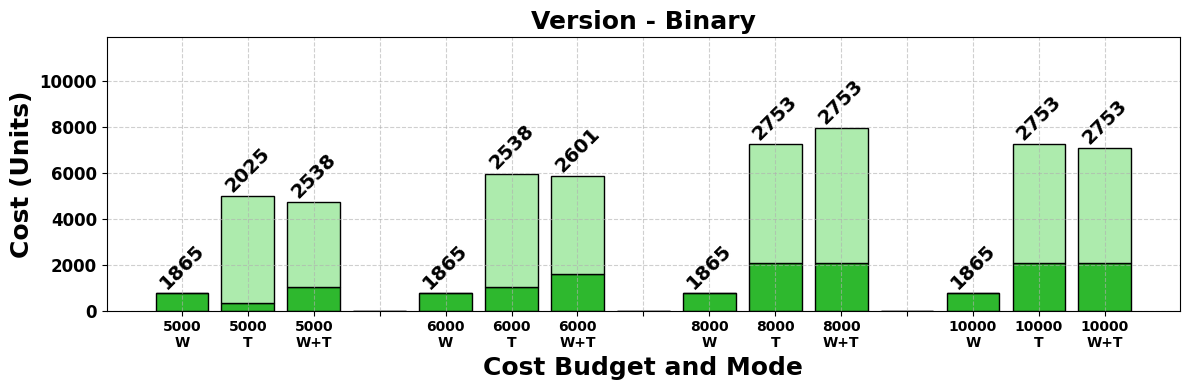
\includegraphics[width=0.5\textwidth]{plots/CU4_pkj.png}
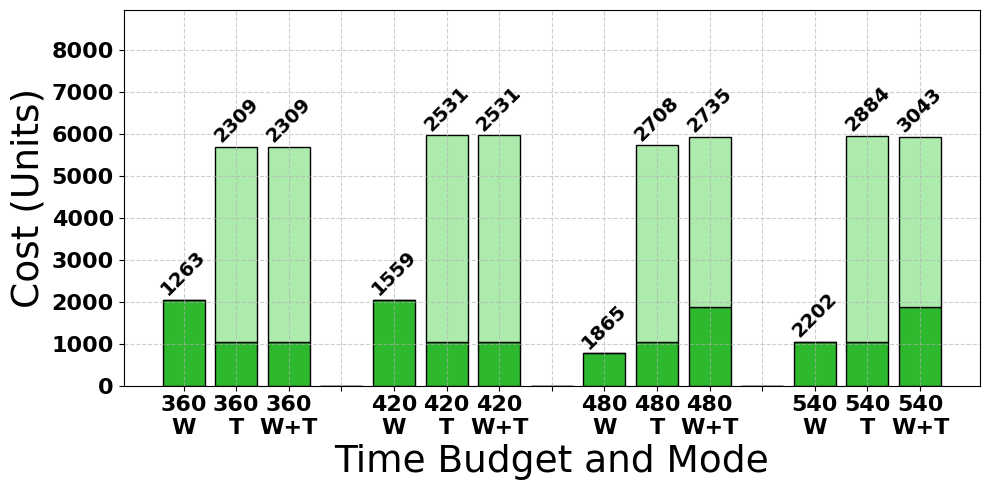
\includegraphics[width=0.5\textwidth]{plots/cu5.png}
% 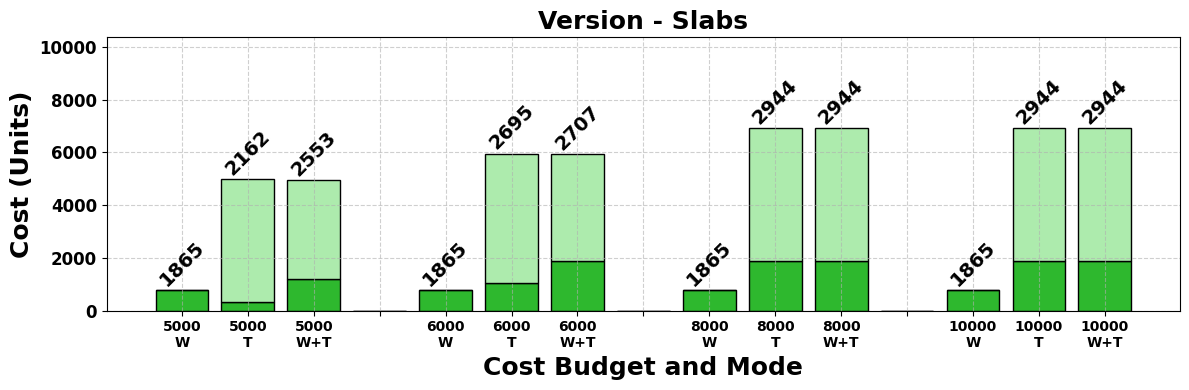
\includegraphics[width=0.5\textwidth]{plots/CU6_pkj.png}
\centering
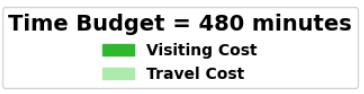
\includegraphics[width=0.3\textwidth]{plots/cu5_legend.png}
\caption{Cost Utilization in 3 travel Modes on different time budgets and fixed time budget (480 minutes)- Osaka}
\label{fig:CostUtilization2}
\end{figure}

These plots in Figures~\ref{fig:CostUtilization1} and ~\ref{fig:CostUtilization2} highlight that in itinerary optimization, cost utilization and utility maximization do not always go hand in hand — the system’s goal is to maximize utility under given constraints rather than simply minimizing or maximizing cost. The entrance (visiting) cost is not directly proportional to the utility score, as some high-utility POIs may have lower entrance costs while others with higher costs may not contribute proportionally to utility. In pure taxi mode, although faster travel allows reaching distant POIs, the high travel cost often exhausts the budget before accessing faraway high-utility POIs, leaving unutilized time. In contrast, the hybrid mode (walking + taxi) leverages walking to access distant, high-utility POIs without incurring excessive travel costs, leading to higher utility even when total cost utilization appears lower. The plots also depict that after a certain threshold, increasing the cost budget yields diminishing returns since time becomes the primary limiting resource.


\noindent\textbf{Utility vs Time budget on different cost budgets}\\

\begin{figure*}[htbp]
    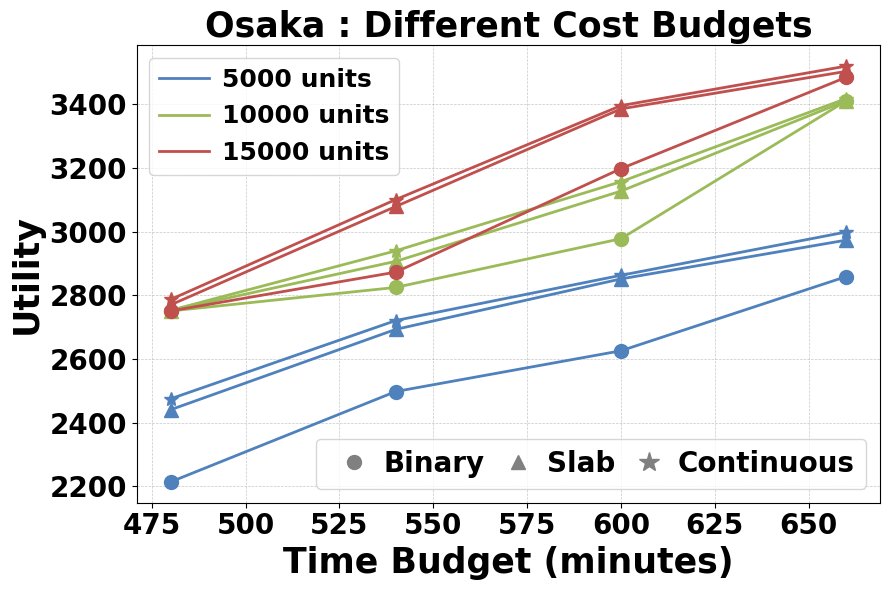
\includegraphics[width=0.33\textwidth]{plots/exp1-osaka.png}
    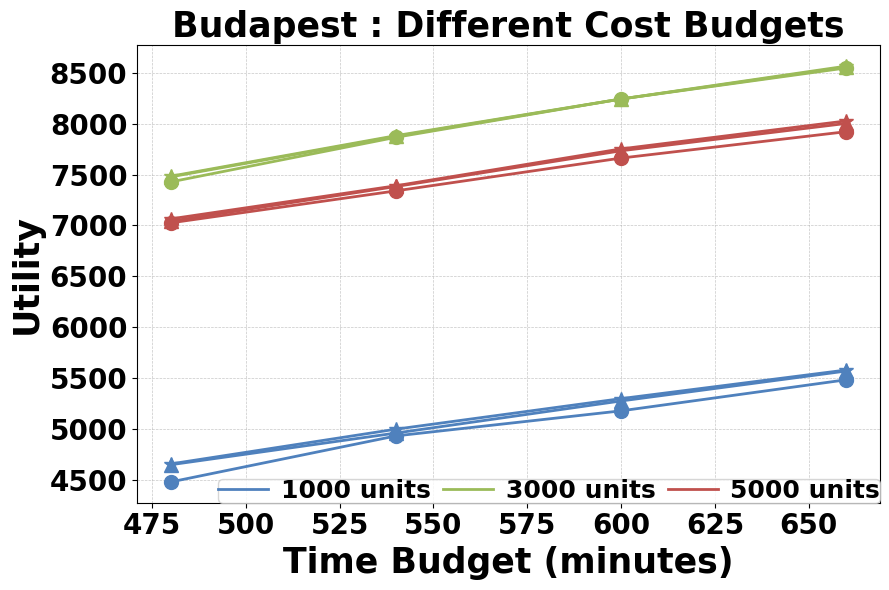
\includegraphics[width=0.33\textwidth]{plots/exp1-budapest.png}
    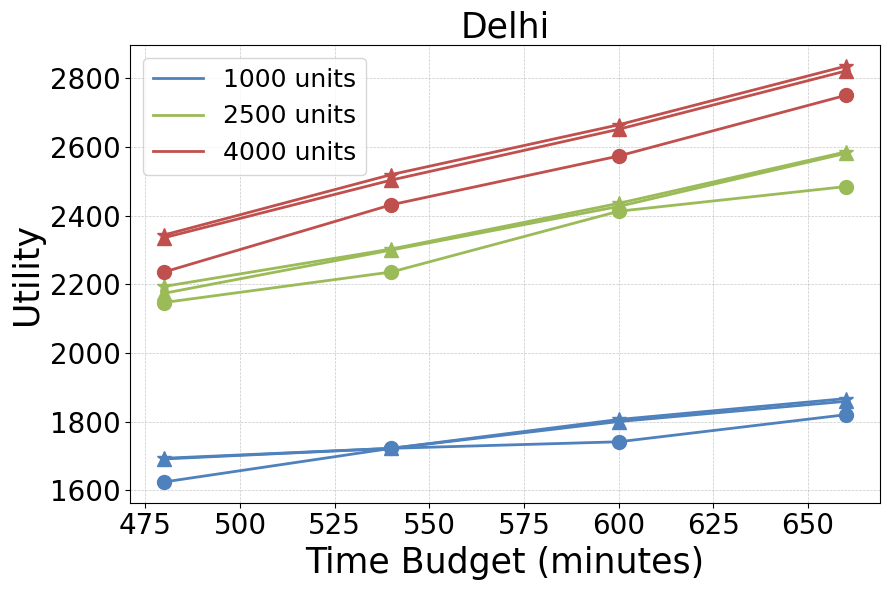
\includegraphics[width=0.33\textwidth]{plots/exp1-delhi.png}
    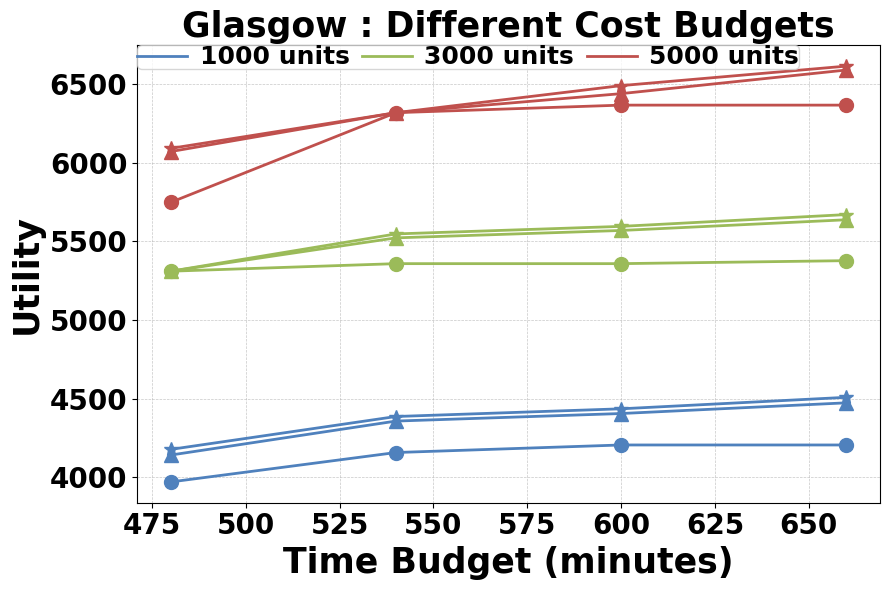
\includegraphics[width=0.33\textwidth]{plots/exp1-glasgow.png}
    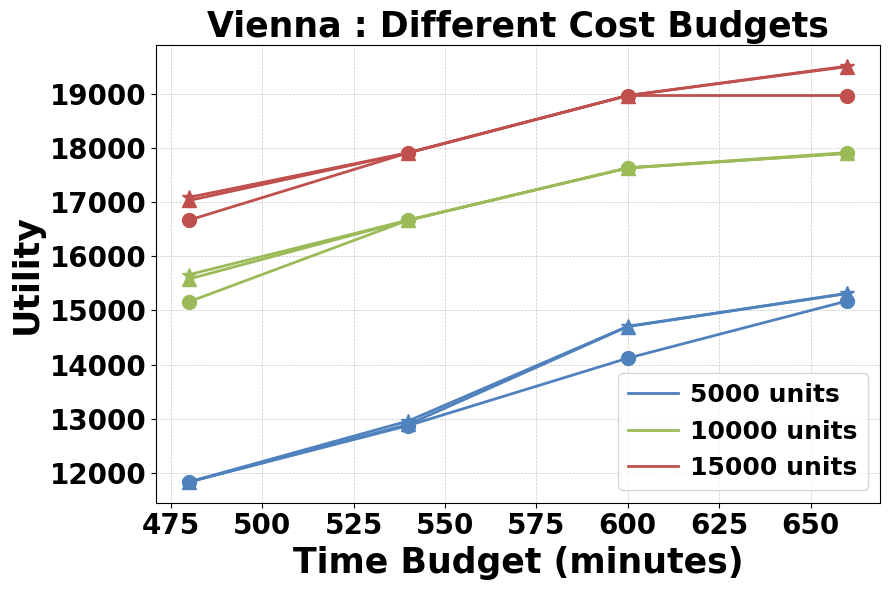
\includegraphics[width=0.33\textwidth]{plots/exp1-vienna.png}
    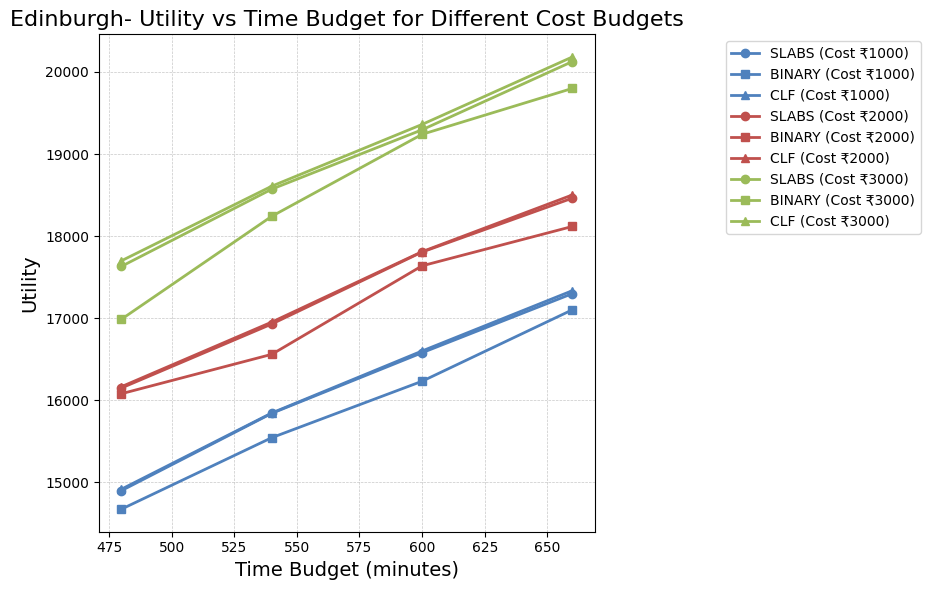
\includegraphics[width=0.33\textwidth]{plots/exp1-edinburgh.png}
    \begin{center}
        
\includegraphics[width=0.6\textwidth]{plots/city_legend.png}
    \end{center}
    \caption{Utility variation with time and cost in 6 cities}
    \label{fig:cities}
\end{figure*}

\noindent \textbf{How to Read the Graphs}

\noindent The graph uses \textbf{colored lines} to represent different \textbf{cost budgets}—for example in Osaka we use blue for 5000 units, green for 10000 units, and red for 15000 units—while \textbf{symbols on the lines} denote different versions of the itinerary planner: squares for \textit{Binary}, triangles for \textit{Slab}, and plus signs for \textit{Continuous Function (CF)}. Each line formed by a specific combination of color and symbol indicates the \textbf{utility trend} for a particular planner variant at a given cost budget. For instance, in Osaka the \textbf{blue line with square markers} represents the performance of the \textit{Binary version} at a \textbf{cost budget of 5000 units}. This combination-based encoding enables a comparative analysis of planner performance across various time and cost constraints.

\noindent\textbf{Insights}

\noindent Figure~\ref{fig:cities} illustrates how the achieved utility varies across different combinations of time and cost budgets for the seven cities in our dataset. A few consistent trends emerge across all cities. First, for a fixed cost budget, increasing the available time consistently leads to higher utility, highlighting the value of longer exploration durations. Second, for a given time budget, allocating a higher cost budget also results in improved utility, indicating the benefit of greater financial flexibility. Most notably, the C variant consistently outperforms both the S and B versions in terms of utility achieved, suggesting its superior effectiveness in balancing constraints across diverse urban scenarios.\\

% % \newpage
% \noindent\textbf{Variation of Utility in Multi-day Itineraries}
% \begin{figure}[th]
% 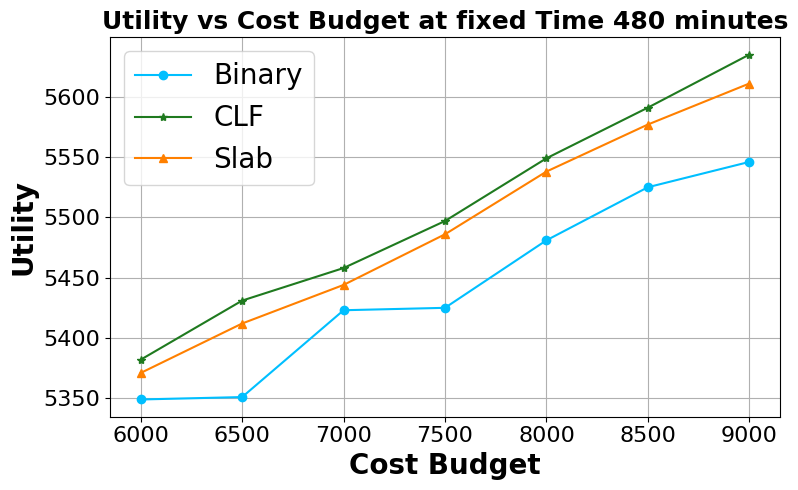
\includegraphics[width=0.45\textwidth]{plots/multiday1_pkj.png}
% % \end{figure}
% % \begin{figure}[th]
% 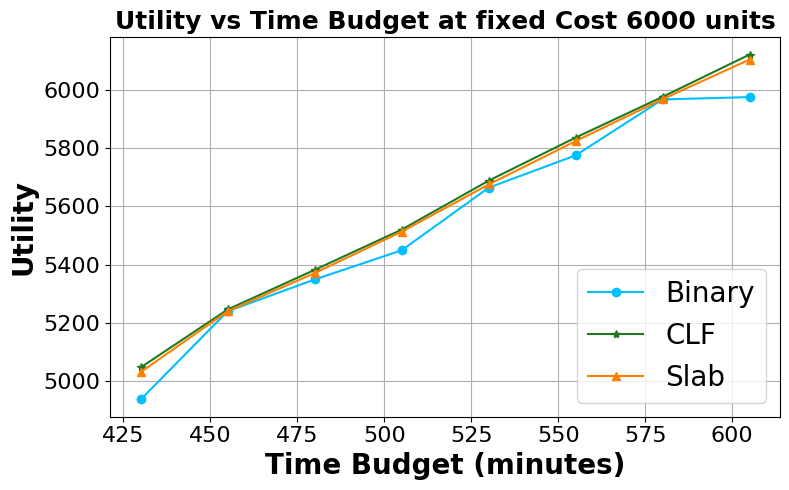
\includegraphics[width=0.45\textwidth]{plots/multiday2_pkj.png}
% \caption{Plots showing trends in Multi-day itineraries (3-day Trip) with Time Budget 480 minutes and Cost Budget 6000 units respectively}
% \label{fig:util_md}
% \end{figure}

% Figure ~\ref{fig:util_md} presents the utility trends for the multi-day variant of our itinerary planner for a 3 day trip. Similar to the single-day analysis, a consistent increasing trend in utility results is observed with fixed cost budget and increasing time budget and vice-versa, across the various formulations. Specifically, the utility achieved using the fractional variant is consistently higher than that of the binary variant, reaffirming the advantages of allowing partial visitations in enhancing overall experience. Furthermore, within the fractional formulations, the CLF (Continuous Linear Fractional) approach typically yields higher utility than the slab-based version, demonstrating its stronger capability to balance constraints and exploit budget flexibility effectively across multiple days of planning. However slabbed version works better than the binary version and thus it can be used to mathematically model the non linear utility functions in our problem which otherwise cannot be handled directly by ILP solvers and thus resulting in a better performance than the binary version.\\

\noindent\textbf{Multi-day Trips vs 3 single day trips}
\begin{figure}[th]
\centering
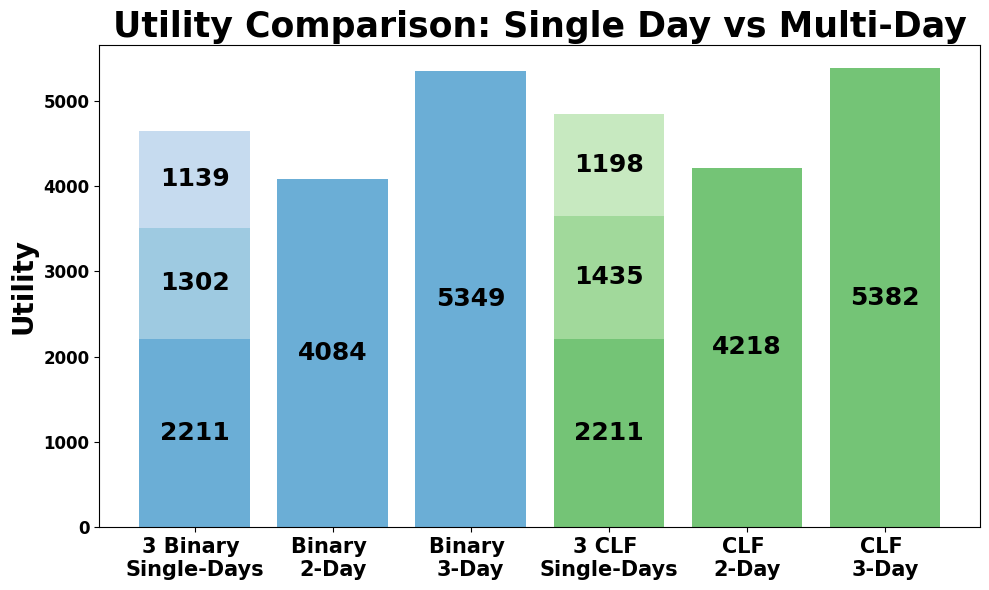
\includegraphics[width=0.45\textwidth]{plots/multivssingle.png}
\caption{Comparison of aggregated Single day trips with 2 day and 3 day multi-day trips}
\label{fig:singlevsmultiday}
\end{figure}
Figure ~\ref{fig:singlevsmultiday}  illustrates a comparison of total utility achieved with different trip planning configurations: aggregated 3 single-day trips versus actual 2-day and 3-day multi-day itineraries, optimized for both Binary and CLF versions. In this experiment, each day was assigned an equal time budget of 480 minutes. For single-day trips, the cost budget was uniformly set at 2000 units per day, and for the multi-day cases, the aggregate cost budgets were similarly scaled: 4000 units for 2-day and 6000 units for 3-day trips. As a basis of comparison, the 3 single day trips were: source-to-hotel travel (bottom segment), hotel-to-destination travel (middle segment), and hotel-to-hotel travel (top segment). The last two segments are swapped for a fair comparison with 2-Day multiday trip version.\\

The results clearly demonstrate that multi-day planning consistently outperforms naive aggregation over single days. In the Binary variant, the 2-day multi-day plan has a score of 4084, whereas two single-day plans aggregated give lower cumulative utility. Similarly, in the 3-day variant, the multi-day plan has a score of 5349, much higher than the three single-day utilities summed up. The same is the case with the CLF variant, where the multi-day plans (4218 for 2-day, 5382 for 3-day) consistently beat the aggregated single-day tallies. This improved performance is due to the flexibility and optimization advantages of multi-day planning, where activities and itineraries can be optimized globally over multiple days as opposed to being restricted within independent daily plans. Thus, multi-day trip planning is not a single-day plan aggregation but a richer solution space that optimally exploits inter-day complementarities.
\noindent\textbf{Effect of personalized constraints on Utility}
\begin{figure}[H]
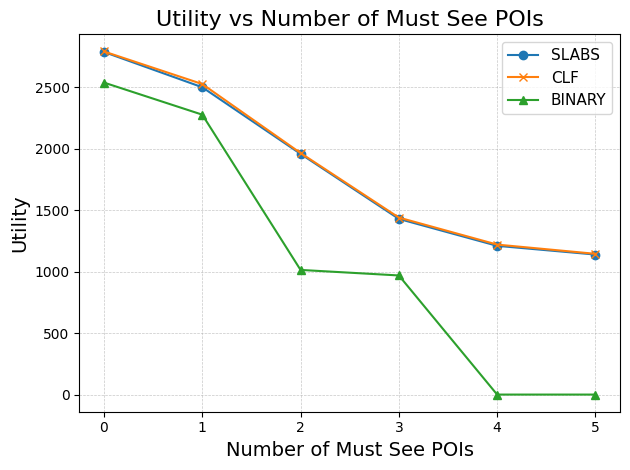
\includegraphics[width=0.24\textwidth]{plots/mustsee.png}
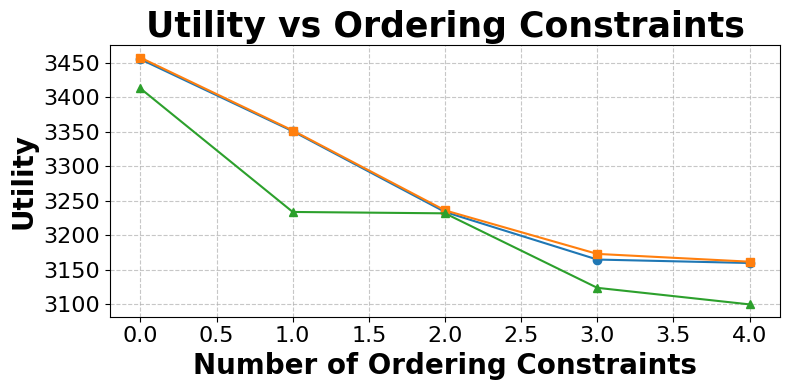
\includegraphics[width=0.24\textwidth]{plots/ordering.png}
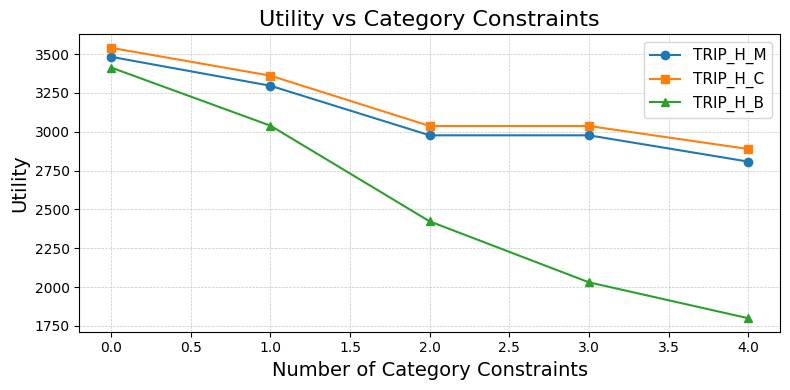
\includegraphics[width=0.24\textwidth]{plots/category.png}
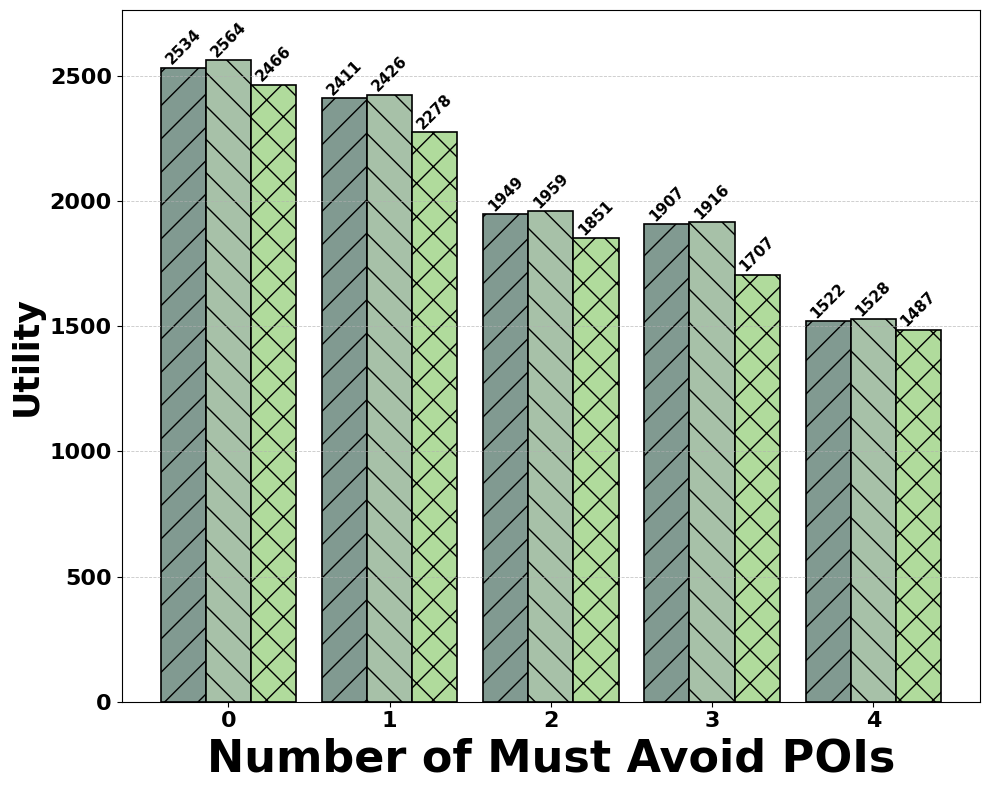
\includegraphics[width=0.24\textwidth]{plots/mustavoid.png}
% \raisebox{0.5\height}{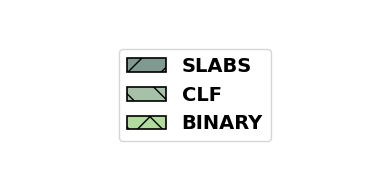
\includegraphics[width=0.24\textwidth]{plots/legend_personalized_pkj.png}}
\caption{Effect of personalized constraints}
\label{fig:personalizedconstraints}
\end{figure}

The impact of incorporating personalized constraints, that is, must-see, ordering, and category constraints, on overall utility is illustrated in the three graphs in figure ~\ref{fig:personalizedconstraints}. In this study a cost budget of 6000 units and a time budget of 480 minutes is utilized and across all cases, it is evident that increasing the number of constraints leads to a decline in the achievable utility, as the solution space becomes more restricted. However, the extent of this reduction varies across the different formulations. Specifically, the CLF and slab variants show a relatively gradual decline in utility compared to the binary variant. This is primarily because the binary model lacks the flexibility to accommodate partial visits to points of interest (POIs), thereby limiting its ability to adapt to tighter constraints. In contrast, the CLF and slab variants can better navigate these constraints by leveraging their ability to assign fractional visits, thus preserving higher utility under increasingly personalized user preferences.\\

\noindent\textbf{Effect of Dynamic Re-routing}
\begin{figure}[th]
    \centering
    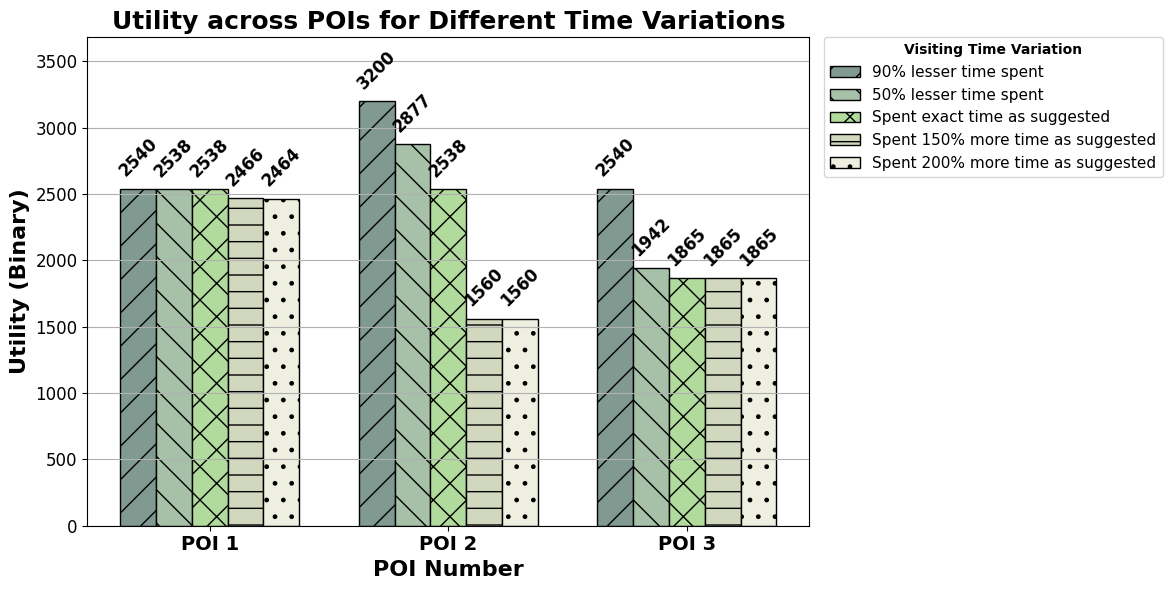
\includegraphics[width=0.50\textwidth]{plots/dynamic_pkj.png}
    \caption{Comparison of utility when tourist gets delayed, reaches on time and arrives early}
    \label{fig:dynamic_pkj}
\end{figure}

% \begin{figure*}[htbp]
%     \centering
%     % 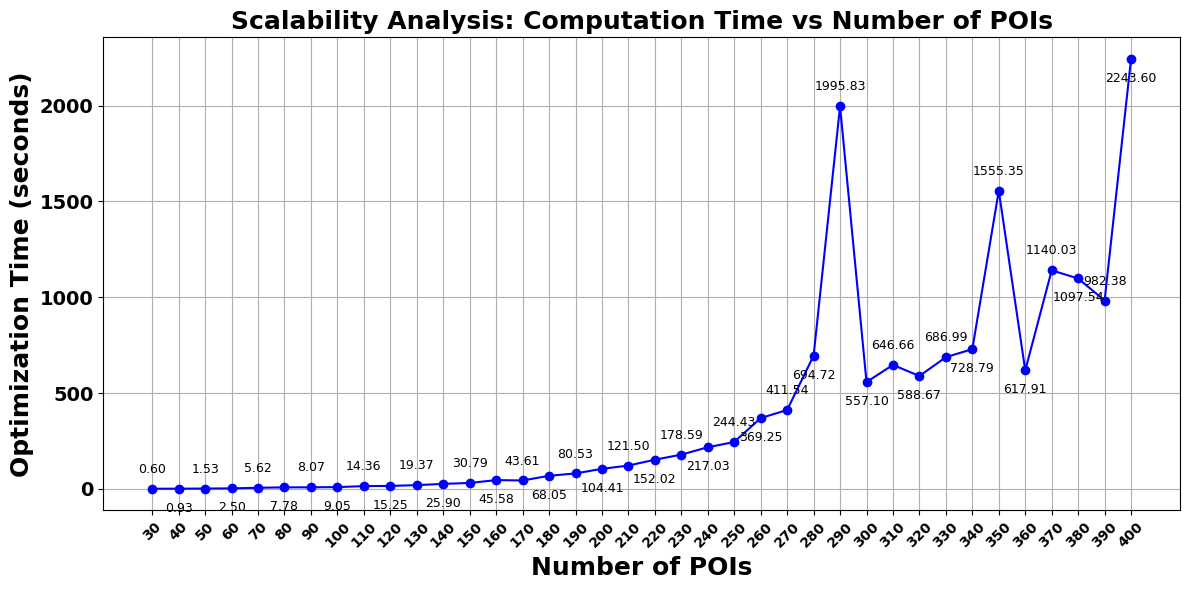
\includegraphics[width=\textwidth]{plots/scalability_pkj.png}
%     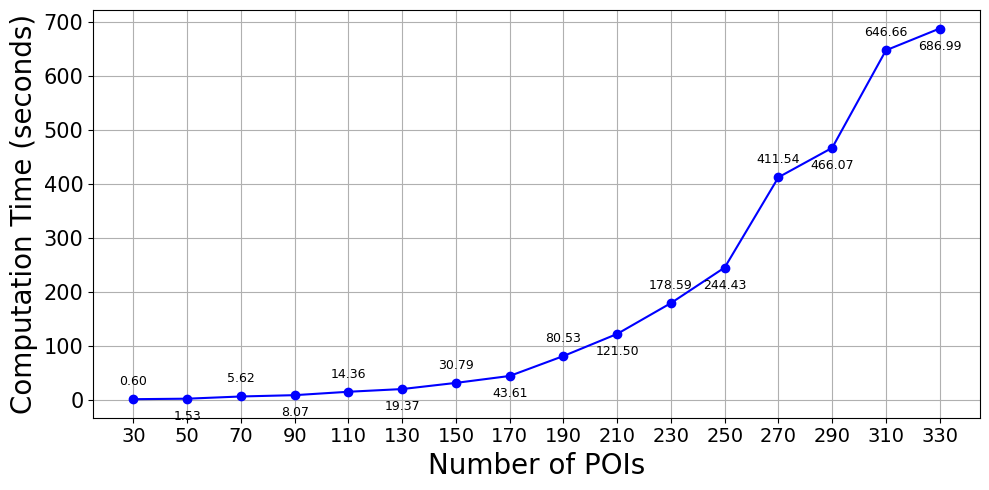
\includegraphics[width=\textwidth]{plots/scalability_new_pkj.png}
%     \caption{Time of computation on increasing number of POIs in single-day trips.}
%     \label{fig:scalability1}
% \end{figure*}

\noindent\textbf{1. How to Read ~\ref{fig:dynamic_pkj}}

This grouped bar chart in Figure ~\ref{fig:dynamic_pkj} compares utility values (Y-axis) for three Points of Interest (POIs) under five different time-spent variations. The five scenarios include: (1) \textit{90\% Less Visiting Time}, where the user spends 90\% lesser time at a POI; (2) \textit{50\% Less Visiting Time}, where the user spends 50\% lesser time at a POI; and (3) \textit{Ontime}, where the user spends the suggested time at all POIs; (4) \textit{150\% More Visiting Time}, where the user spends 150\% more time at a POI; (5) \textit{200\% More Visiting Time}, where the user spends 200\% more time at a POI. 
In all cases, travel times between any pair of POIs remain unaffected by user behaviour, and it takes the same time to travel by the user as suggested. Each POI has five bars, each representing a scenario from spending 90\% less time to 200\% more time than suggested at that POI. Bar heights indicate utility levels, with values labeled on top. Distinct patterns and colors differentiate time-spent categories, as indicated in the legend.\\

\noindent\textbf{2. Insights}

Our planner dynamically recalculates the itinerary by considering the actual time a user spends at each Point of Interest (POI) and the time taken to travel between them, in contrast to the initially suggested schedule.  As shown in figure, at a time budget of 480 minutes and cost budget of 6000 units in TRIP\_H\_B variant, the \textbf{utility consistently decreases} as the time spent at a POI increases.

This trend can be explained as follows:

\begin{itemize}
    \item Spending \textbf{less time} at a POI allows the user to \textbf{save time}, which can be used to visit \textbf{additional POIs}, thereby increasing the overall utility.
    \item Conversely, as more time is spent at a single POI, the user has \textbf{less time available} to explore other POIs, resulting in a \textbf{decrease in total utility}.
\end{itemize}

\noindent This variation in utility values underscores the importance of adapting the itinerary based on real-time user behavior, demonstrating the effectiveness of our dynamically responsive planning approach.\\

\noindent\textbf{Conclusion}

\ab{Please read this section!}\\
As shown in Figure~5, we are able to successfully replicate the existing baseline version presented in this paper for single-day trip planning using our binary walking version of the itinerary planner (\texttt{TRIP\_W\_B}). Furthermore, our other variants of the itinerary planner consistently outperform the existing baseline. Therefore, the baseline is dropped from any other analysis.

Moving forward, as observed in all the figures of this section, both the Continuous and Slab variants of the itinerary planner demonstrate superior performance over the Binary variant by enabling users to achieve higher utility values. This provides sufficient evidence to establish that the Continuous and Slab variants are more effective than the Binary variant, and hence, the study is continued with these two versions only. However, while the Continuous variant generally yields higher utility compared to the Slab variant, it is not appropriate to directly compare these two approaches. The Slab variant was specifically introduced to address the challenge of modeling non-linear utility functions, which cannot be directly handled by ILP solvers. By discretizing such non-linear functions into multiple slabs, they can be mathematically formulated and optimized within the ILP framework. Therefore, Continuous and Slab variants serve distinct purposes and address different problem complexities; any direct comparison in terms of utility alone would be misleading. Both variants offer unique advantages in handling different utility modeling scenarios, and hence, we continue the subsequent analysis with both, without declaring either one superior over the other.
 
\noindent\textbf{Scalability}\\
To evaluate the scalability of our itinerary planning system, we examine how the computation time required to generate a complete itinerary varies with the number of Points of Interest (POIs) in a city, while keeping the time and cost budgets fixed at sufficiently accommodating values of 480 minutes and 6000 units respectively. As illustrated in Figure~\ref{fig:dynamic}, the observed increase in computation time with the number of POIs is expected, given that our approach is formulated as an Integer Linear Program (ILP). This growth aligns with the theoretical complexity of the underlying problem — a variant of the Team Orienteering Problem — which is known to be NP-Hard. Despite this, our formulation remains tractable for problem sizes typical of real-world tourist cities. Despite this theoretical complexity, our system demonstrates strong practical performance. For instance, with approximately 180 POIs, the itinerary is generated in under 1 minute. Even with nearly 260 POIs, the computation time remains approximately 5 minutes. These results highlight that, for realistically sized cities, our system maintains high computational efficiency, making it a viable and scalable solution for real-world deployment.

\begin{figure}[H]
    \centering
    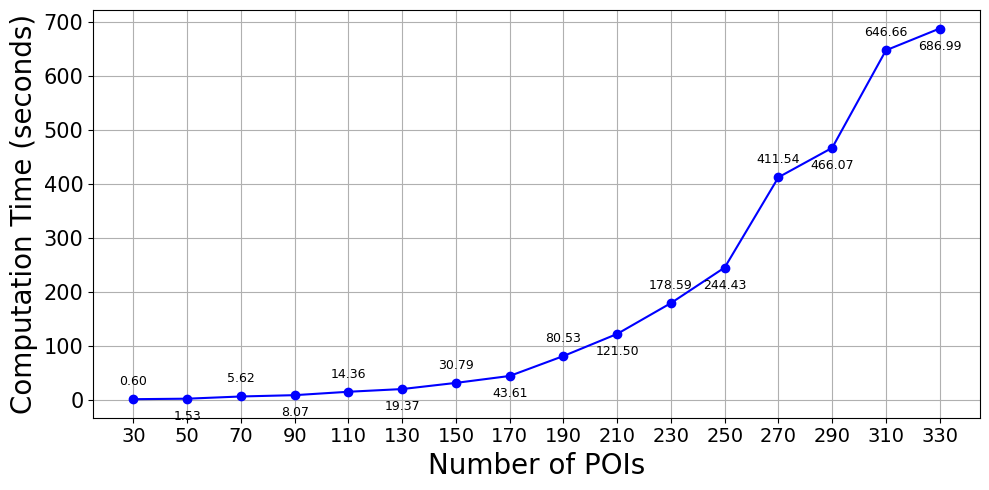
\includegraphics[width=0.50\textwidth]{plots/scalability_new_pkj.png}
    \caption{Comparison of utility when tourist gets delayed, reaches on time and arrives early}
    \label{fig:dynamic}
\end{figure}

In order to further check the scalability of the suggested itinerary planning system, we designed an experiment by increasing the number of days in the trip as shown in ~\ref{fig:scalability2}. The time budget was chosen as 480 minutes per day and the cost budget for day 1 was kept 2000 units for the whole trip. We kept increasing the cost budget by 2000 units on each subsequent day. The experiment was run for trips from 1 to 6 days.

The Time of Computation (TOC) for each case was measured. As anticipated, the TOC grows large as the days increase, mostly owing to the exponential increase in the solution space with the more days. It thereby aptly captures the scalability issue presented by multi-day travel itinerary planning and highlights the necessity for efficient optimization methods in processing longer trip durations.\\

\begin{figure}[th]
    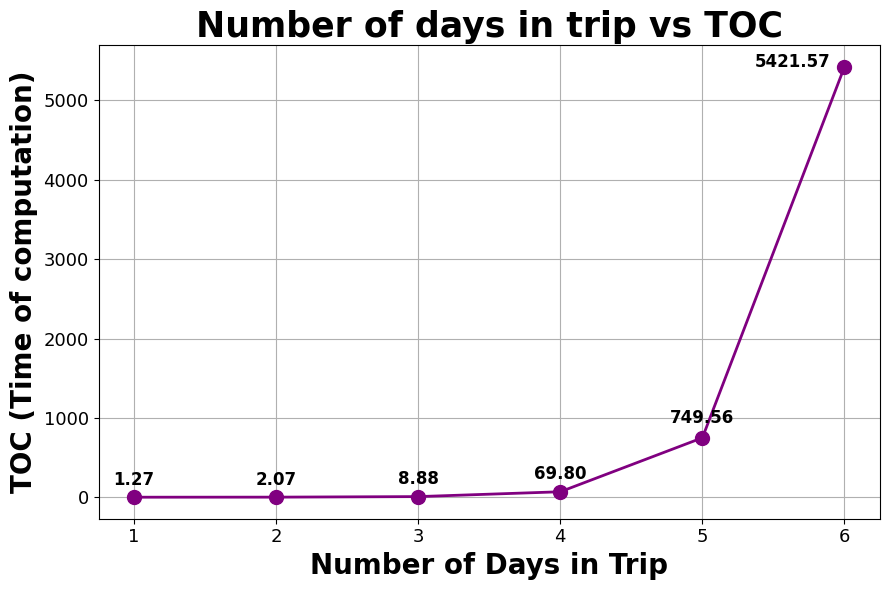
\includegraphics[width=0.5\textwidth]{plots/multidayvstoc.png}
     \caption{Time of computation on increasing number of days in multi-day trips}
    \label{fig:scalability2}
\end{figure}


% \begin{figure*}[htbp]
%     \centering
%     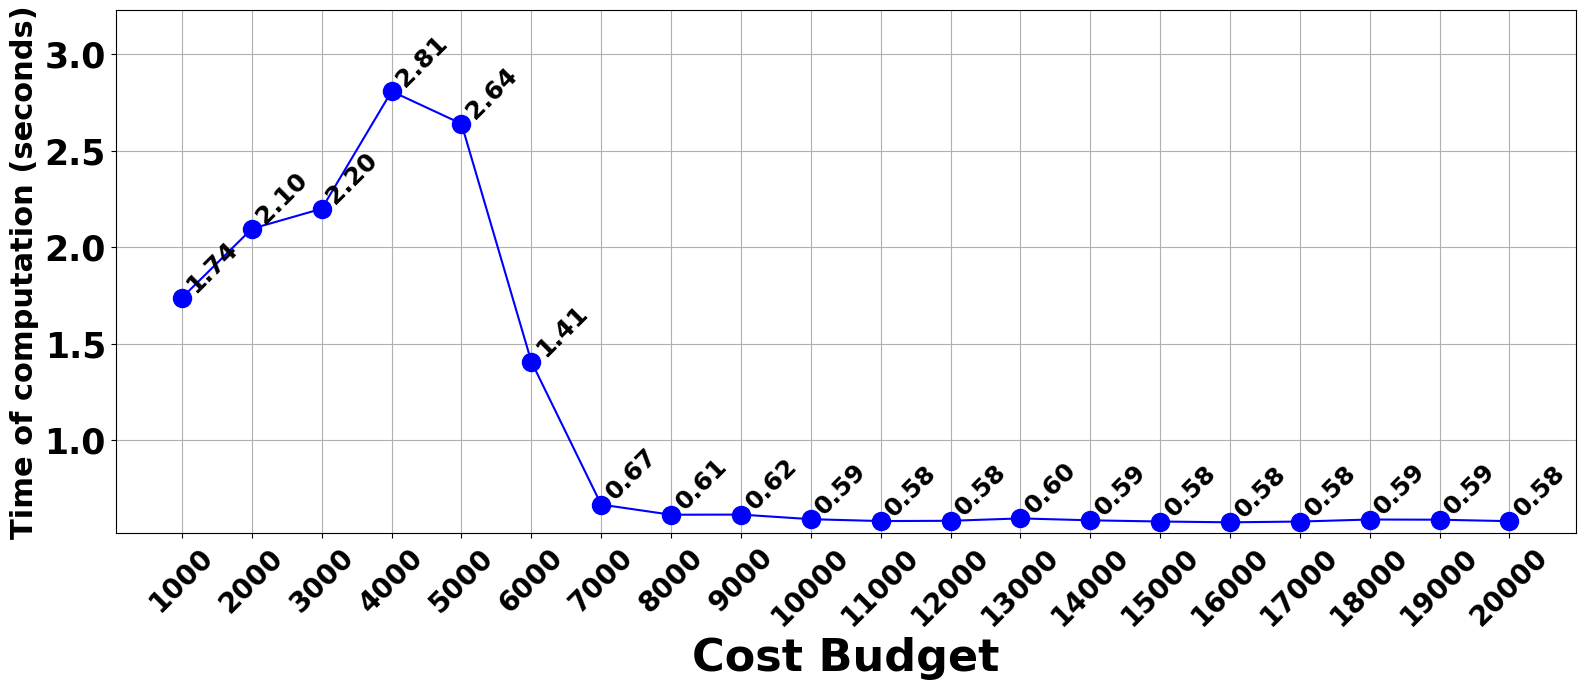
\includegraphics[width=\textwidth]{plots/costbudgetvstoc.png}
%     \caption{Time of computation on increasing cost budget at fixed time budget 480 minutes}
%     \label{fig:costbudgetvstoc}
% \end{figure*}



% \begin{figure*}[htbp]
%     \centering
%     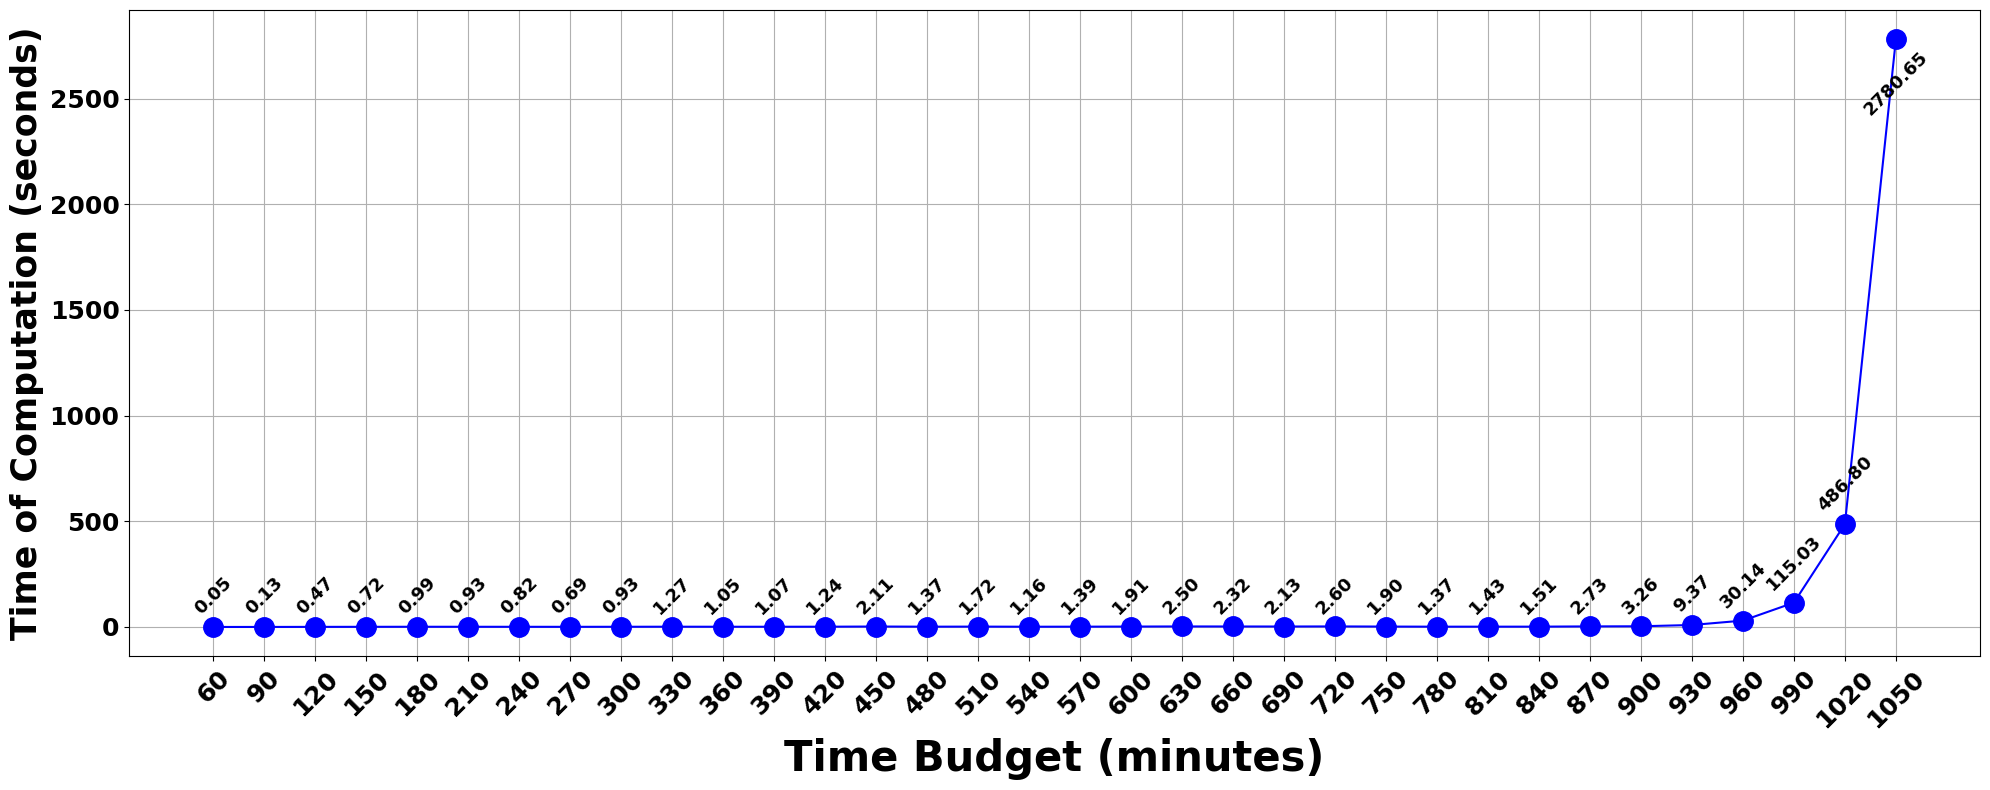
\includegraphics[width=\textwidth]{plots/timebudgetvstoc.png}
%     \caption{Time of computation on increasing time budget at fixed cost budget 6000 units}
%     \label{fig:timebudgetvstoc}
% \end{figure*}



\noindent The computational efficiency of the suggested itinerary optimization model was tested against both cost budget and time budget changes. In figure~\ref{fig:costbudgetvstoc}, as the cost budget rises from low values, the computation time records a minimal increment and hits a plateau, perhaps as the solution space complexity is raised. But above some cost budget limit (approximately 6000), the computation time levels off and is always low for a broad range of cost budgets. This indicates that after the feasible space is large enough, further increases in the budget no longer have a major effect on solver performance. On the contrary, figure~\ref{fig:timebudgetvstoc} illustrates that computation time is much less robust to the time budget. Though initial time budget increases cause only incremental increases in computation time, after about 900 minutes, the solver time becomes steeply exponentially increasing, reflecting the growing challenge of searching a very much larger feasible space. Particularly towards the upper end, computation time skyrockets, pointing out that cost budget is less important than time budget in defining the computational complexity of the problem.

\begin{figure}[H]
    \centering
    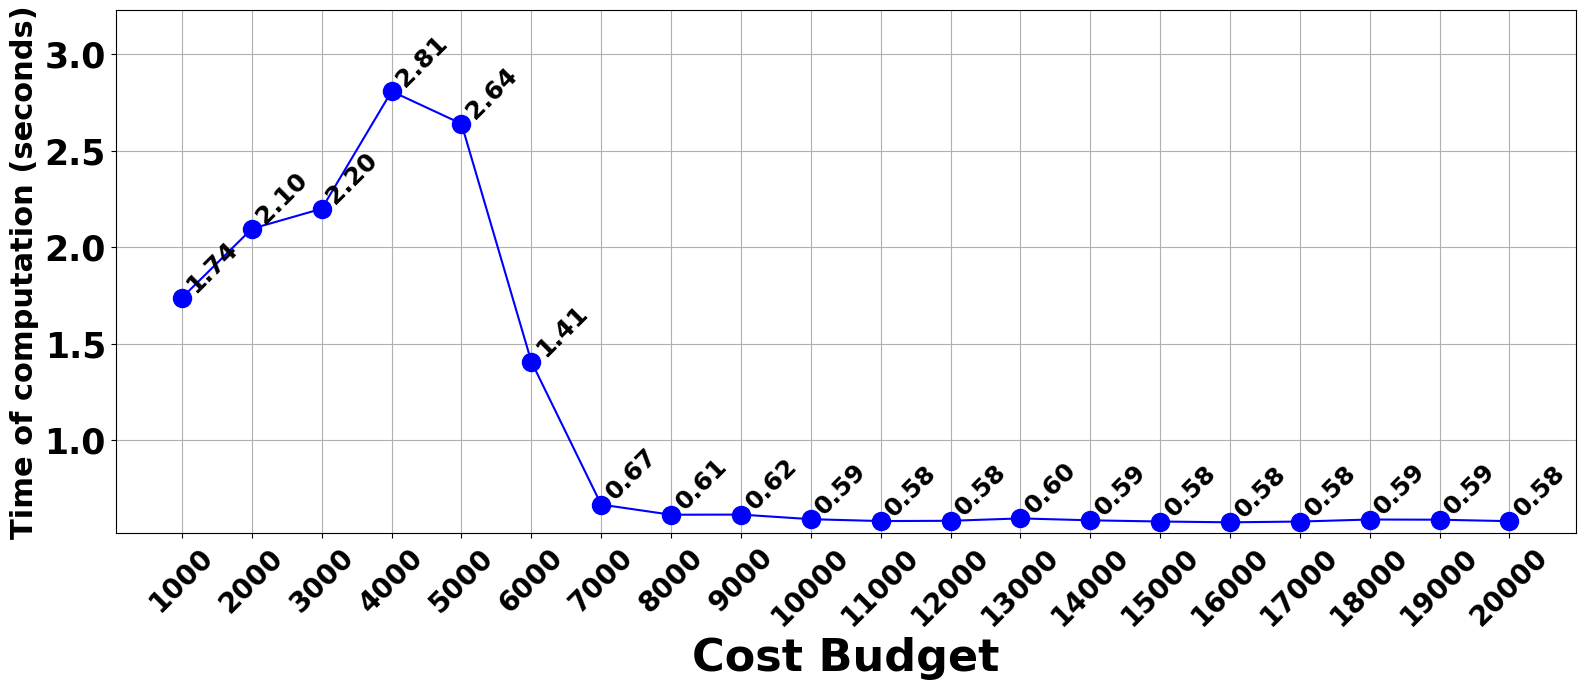
\includegraphics[width=0.50\textwidth]{plots/costbudgetvstoc.png}
    \caption{Time of computation on increasing cost budget at fixed time budget 480 minutes}
    \label{fig:costbudgetvstoc}
\end{figure}

\begin{figure}[H]
    \centering
    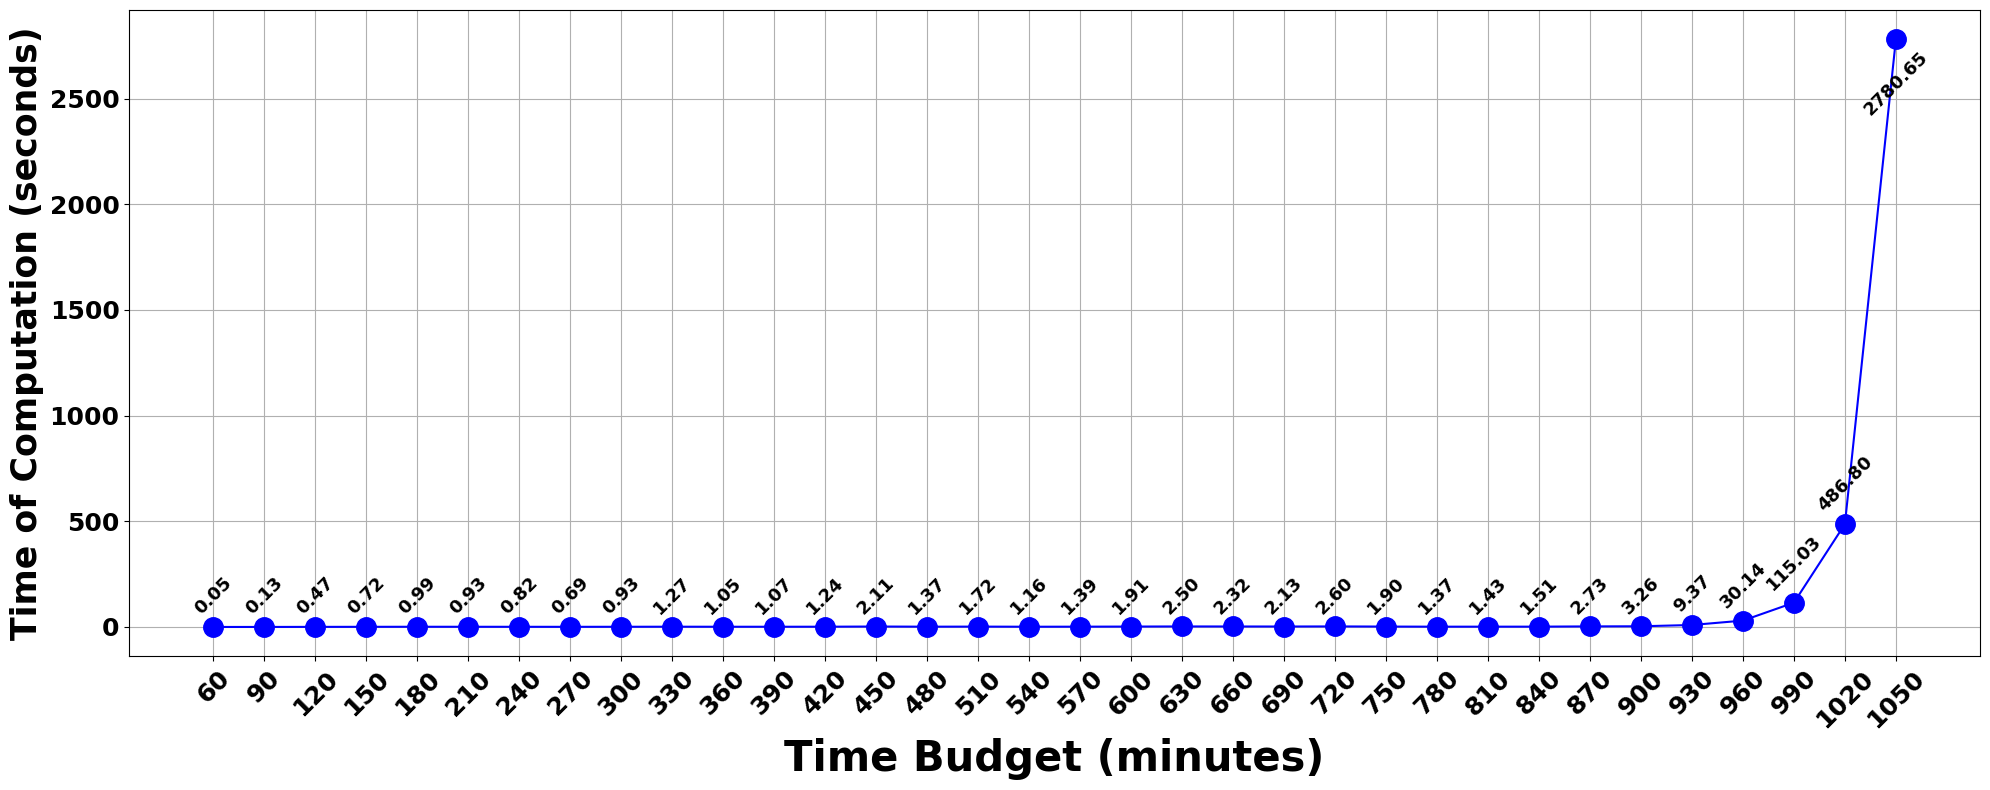
\includegraphics[width=0.50\textwidth]{plots/timebudgetvstoc.png}
    \caption{Time of computation on increasing time budget at fixed cost budget 6000 units}
    \label{fig:timebudgetvstoc}
\end{figure}
\section{Conclusions and Future Work}
\label{Conclusions}

This paper revisits the trip itinerary planning problem and proposes a novel solution framework called \trip that returns an \emph{optimal itinerary} as a solution for practical scenarios. This solution allows multi-day itinerary planning that not only considers the tourist's starting and ending locations and timings, but also adheres to the operational timings of each POI. The proposed solution is unique and powerful due to its ability to accommodate multiple transportation modes, factoring of user-specified personalized constraints such as must-see constraints, must-avoid constraints, ordering constraints and category constraints, consideration of multiple utility variants, and the capability of dynamic re-planning of the itinerary to account for unplanned delays or early exits experienced during the previously visited POIs. Empirical evaluation on several popular destinations show the efficacy and efficiency of the proposed solution.

In future, other transportation modes such as cycle, public bus and metro can be considered. Further, real-time crowd and resulting waiting times at each POI can be factored to generate more useful itineraries.


\pagebreak

%\section*{AI-Generated Content Acknowledgement}

%We have used the generative artificial intelligence (GenAI) tool ChatGPT for help in paraphrasing and small edits.

\bibliographystyle{ACM-Reference-Format}
%\bibliographystyle{IEEEtranS}
\balance
\bibliography{references}

\end{document}

